\begin{frame}{Types of Payouts to Shareholders}
\footnotesize
\begin{itemize}
    \item \textbf{Cash Dividends} -- The most common form:
    \begin{itemize}
        \item \textit{Regular cash dividend}: Typically paid quarterly in the U.S.
        \item \textit{Extra dividend}: Paid occasionally when the firm has surplus cash.
        \item \textit{Liquidating dividend}: A one-time payout as the firm winds down.
    \end{itemize}

    \item \textbf{Stock Dividends} -- Paid in the form of additional shares:
    \begin{itemize}
        \item No cash leaves the firm.
        \item Dilutes the ownership percentage but not value.
    \end{itemize}

    \item \textbf{Dividends in Kind} -- Non-cash distribution (rare):
    \begin{itemize}
        \item Example: Wrigley's Gum once sent chewing gum to shareholders.
    \end{itemize}

    \item \textbf{Stock Buybacks} -- An alternative to dividends:
    \begin{itemize}
        \item Reduces the number of shares outstanding.
        \item Can signal undervaluation or distribute temporary cash flows flexibly.
    \end{itemize}
\end{itemize}
\end{frame}

\subsection{Cash Dividend}
\subsubsection{Timeline}
\begin{frame}{Timeline of a Cash Dividend Payment}
\begin{figure}
    \centering
    
\includegraphics[width=0.9\textwidth]{images/section5/dividendprocess}
\end{figure}
\vspace{-5mm}
\footnotesize
\begin{itemize}
    \item \textbf{Declaration Date}: The board announces the dividend (a legal liability is created).
    \item \textbf{Record Date}: Shareholders on record at this date are entitled to receive the dividend.
    \item \textbf{Ex-Dividend Date}: Typically two business days before the record date. Buyers on or after this date will \textit{not} receive the dividend.
    \item \textbf{Cum-Dividend Date}: The last day when a buyer of the stock still receives the dividend.
    \item \textbf{Payment Date}: The date when dividend checks are mailed or direct deposits made.
\end{itemize}
\end{frame}

\begin{frame}{Apple Inc. (AAPL) Dividend History: 2022-2024}
\footnotesize
\begin{table}[h]
\centering
\resizebox{\textwidth}{!}{
\begin{tabular}{cccccc}
\toprule
\textbf{Ex-Date} & \textbf{Type} & \textbf{Amount} & \textbf{Declaration Date} & \textbf{Record Date} & \textbf{Payment Date} \\
\midrule
05/10/2024 & Cash & \$0.25 & 05/02/2024 & 05/13/2024 & 05/16/2024 \\
02/09/2024 & Cash & \$0.24 & 02/01/2024 & 02/12/2024 & 02/15/2024 \\
11/10/2023 & Cash & \$0.24 & 11/02/2023 & 11/13/2023 & 11/16/2023 \\
08/11/2023 & Cash & \$0.24 & 08/03/2023 & 08/14/2023 & 08/17/2023 \\
05/12/2023 & Cash & \$0.24 & 05/04/2023 & 05/15/2023 & 05/18/2023 \\
02/10/2023 & Cash & \$0.23 & 02/02/2023 & 02/13/2023 & 02/16/2023 \\
11/04/2022 & Cash & \$0.23 & 10/27/2022 & 11/07/2022 & 11/10/2022 \\
08/05/2022 & Cash & \$0.23 & 07/28/2022 & 08/08/2022 & 08/11/2022 \\
05/06/2022 & Cash & \$0.23 & 04/28/2022 & 05/09/2022 & 05/12/2022 \\
02/04/2022 & Cash & \$0.22 & 01/27/2022 & 02/07/2022 & 02/10/2022 \\
\bottomrule
\end{tabular}
}
\end{table}
\vspace{-2mm}
{\tiny Source: NASDAQ}
\end{frame}
\subsubsection{Price Behavior}
\begin{frame}{Price Behavior Around the Ex-Dividend Date}

\small
\textbf{In theory:}  
\vspace{1mm}
\begin{itemize}
    \item In a frictionless market, a stock's price should drop by exactly the amount of the dividend on the \textbf{ex-dividend date}.
\end{itemize}

\vspace{-2mm}
\begin{figure}
    \centering
    
\includegraphics[width=0.75\textwidth]{images/section5/pricebehavior}
\end{figure}
\vspace{-7mm}
\textbf{In practice:}
\begin{itemize}
    \item The price drop is typically \textit{less than the dividend}.
    \item The adjustment usually occurs within minutes of the market opening.
    \item This deviation is primarily due to \textbf{tax preferences} and market microstructure.
\end{itemize}
\end{frame}

\subsubsection{The Irrelevance of Dividend Policy}
\begin{frame}{The Irrelevance of Dividend Policy}

\begin{itemize}
    \item In a perfect capital market, \textbf{dividend policy is irrelevant} to firm value.
    \vspace{2mm}
    \item Investors can create their preferred cash flow stream through \textbf{homemade dividends}:
    \begin{itemize}
        \item Need cash? Sell shares.
        \item Don't want cash? Reinvest dividends.
    \end{itemize}
    \vspace{2mm}
    \item As long as the firm's \textbf{investment policy and total cash flow} remain unchanged, payout decisions do not affect value.
\end{itemize}

\end{frame}

\begin{frame}{Benchmark Case: Bristol Corporation}

\begin{itemize}
    \item Consider a firm with no growth and no investment opportunities.
    \item Bristol Corp. has \$10,000 in cash today and expects \$10,000 more next year, after which it will liquidate.
\end{itemize}

\vspace{3mm}
\begin{center}
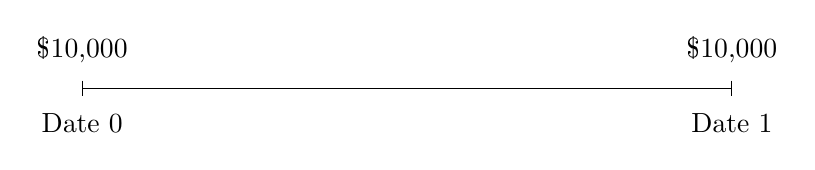
\begin{tikzpicture}[x=1.5cm, y=1cm]
    \draw[-] (0,0) -- (5.5,0);
    \foreach \x in {0,5.5} {
        \draw (\x,0.1) -- (\x,-0.1);
    }
    \node[below] at (0,-0.2) {Date 0};
    \node[below] at (5.5,-0.2) {Date 1};
    \node[above] at (0,0.2) {\$10,000};
    \node[above] at (5.5,0.2) {\$10,000};
\end{tikzpicture}
\end{center}

\begin{itemize}
    \item Discount rate: 10\%
\end{itemize}

\end{frame}

\begin{frame}{Current Policy: Dividend Equals Current Cash Flow}

\begin{itemize}
    \item The firm pays out \$10,000 immediately, and \$10,000 next year.
    \item Present value of the firm:
    \[
        V_0 = \$10,000 + \frac{\$10,000}{1.1} = \$19,090.91
    \]
    \item With 1,000 shares outstanding:
    \[
        P_0 = \$10 + \frac{\$10}{1.1} = \$19.09
    \]
    \item After the dividend, the share price falls to:
    \[
        P_{\text{ex-div}} = \$19.09 - 10 = \$9.09
    \]
\end{itemize}

\end{frame}

\begin{frame}{Alternative Policy: Dividends Greater Than Cash Flow}

\begin{itemize}
    \item Suppose the firm pays a dividend of \$11 per share today.
    \item To finance the extra \$1,000, it issues new equity at \$19.09/share.
    \item New investors expect:
    \[
        \$1,000 \times 1.1 = \$1,100 \text{ return at Date 1}
    \]
    \item Remaining \$8,900 goes to old shareholders:
    \[
        P_0 = \$11 + \frac{\$8.90}{1.1} = \$19.09
    \]
\end{itemize}

\end{frame}

\begin{frame}{The Dividend Indifference Proposition}

\begin{itemize}
    \item Dividend policy does not affect share value if:
    \begin{itemize}
        \item The firm pays out all cash eventually
        \item Capital markets are perfect (no taxes, no transaction costs)
    \end{itemize}
    
    \vspace{2mm}
    \item Investors are indifferent between:
    \begin{itemize}
        \item \textbf{Dividends vs. Capital Gains}: Delayed payouts $\approx$ capital gains
        \item \textbf{Dividends vs. Retained Earnings}: Retained earnings must eventually be distributed
    \end{itemize}
    
    \vspace{2mm}
    \item Homemade dividends replicate any desired cash flow stream
\end{itemize}

\end{frame}

\subsubsection{Homemade Dividends}
\begin{frame}{Homemade Dividends: Investor Preferences}

\begin{itemize}
    \item Investors can adjust their own cash flows to suit their preferences -- regardless of the firm's dividend policy.
    \vspace{3mm}
    
    \item \textbf{Case 1: Investor X prefers smooth dividends of \$10 at Date 0 and Date 1.}
    \begin{itemize}
        \item The firm pays \$11 at Date 0 and \$8.90 at Date 1.
        \item Investor X reinvests the excess \$1 at 10\% return $\rightarrow$ receives \$1.10 at Date 1.
    \end{itemize}
    
    \pause
    \item \textbf{Case 2: Investor Z prefers more income at Date 0 -- e.g., \$11 now and \$8.90 later.}
    \begin{itemize}
        \item Firm pays only \$10 per share today.
        \item Share price after dividend is \$9.09.
        \item To increase current income by \$100, Investor Z sells $\frac{\$100}{\$9.09} \approx 11$ shares.
        \item The remaining 89 shares yield \$8.90 each next year $\rightarrow$ desired total income stream achieved.
    \end{itemize}
\end{itemize}

\end{frame}

\begin{frame}{Homemade Dividends: Indifference Curve}
\begin{center}
    \resizebox{0.8\textwidth}{!}{
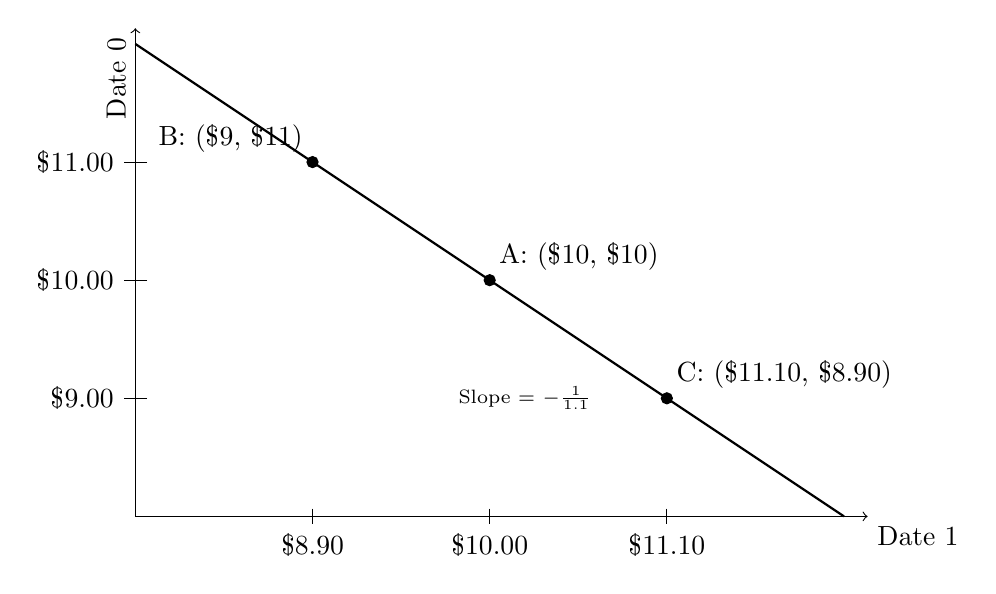
\begin{tikzpicture}[x=1.5cm, y=1cm]
    % Axes
    \draw[->] (0,0) -- (6.2,0) node[below right] {Date 1};
    \draw[->] (0,0) -- (0,6.2) node[above left, rotate=90] {Date 0};

    % Budget constraint line
    \draw[thick] (0,6) -- (6,0);

    % Key points
    \filldraw (3,3) circle (2pt) node[above right] {A: (\$10, \$10)};
    \filldraw (4.5,1.5) circle (2pt) node[above right] {C: (\$11.10, \$8.90)};
    \filldraw (1.5,4.5) circle (2pt) node[above left] {B: (\$9, \$11)};
    
    % Slope annotation
    \node at (3.3,1.5) {\scriptsize Slope = $-\frac{1}{1.1}$};

    % Ticks and labels
    \foreach \x/\xlabel in {1.5/\$8.90, 3/\$10.00, 4.5/\$11.10} {
        \draw (\x,0.1) -- (\x,-0.1) node[below] {\xlabel};
    }
    \foreach \y/\ylabel in {1.5/\$9.00, 3/\$10.00, 4.5/\$11.00} {
        \draw (0.1,\y) -- (-0.1,\y) node[left] {\ylabel};
    }

\end{tikzpicture}
}
\end{center}

\begin{itemize}
    \item Investors can freely move along the \textbf{budget line} by buying or selling shares to adjust the timing of cash flows.
    \item Point A: Firm policy $\rightarrow$ \$10 now and \$10 later.
    \item Point C: Preference for more cash now, offset by lower future income.
\end{itemize}

\end{frame}

\subsubsection*{Cash Dividend Summary}
\begin{frame}{Dividends and Investment Policy: Key Insight}

\begin{itemize}
    \item Increasing dividends by issuing new equity \textbf{does not create value} for shareholders.
    
    \item Reducing dividends through share repurchases \textbf{also does not destroy value}, assuming no change in total cash flow.

    \vspace{3mm}
    \item \textbf{Core Assumption:}
    \begin{itemize}
        \item The firm's overall cash flow level is fixed.
        \item The firm continues to accept all available \textbf{positive NPV projects}.
    \end{itemize}

    \vspace{3mm}
    \item \textbf{Golden Rule:}
    \begin{block}{}
        \centering
        \textit{A firm should never sacrifice a positive NPV investment just to increase or initiate a dividend.}
    \end{block}
\end{itemize}

\end{frame}

\subsection{Repurchase of Stock}
\begin{frame}{Repurchase of Stock: An Alternative to Dividends}

\begin{itemize}
    \item Instead of paying cash dividends, firms may choose to return excess cash via \textbf{share repurchases}.
    \item In a repurchase, the firm buys back its own shares, reducing the number of shares outstanding.
    
    \vspace{2mm}
    \item \textbf{Methods of Share Repurchase}:
    \begin{itemize}
        \item \textit{Open Market Repurchase}: Buy shares on the market like any investor.
        \item \textit{Tender Offer}: Offer to buy a specific number of shares at a premium.
        \item \textit{Dutch Auction}: Shareholders state prices; firm accepts the lowest prices that fulfill its target.
        \item \textit{Private Negotiation} (Greenmail): Buy back from large investors under negotiated terms.
    \end{itemize}
\end{itemize}

\end{frame}

\begin{frame}{Earnings, Dividends, and Buybacks for Large U.S. Firms}

\begin{figure}
    \centering
    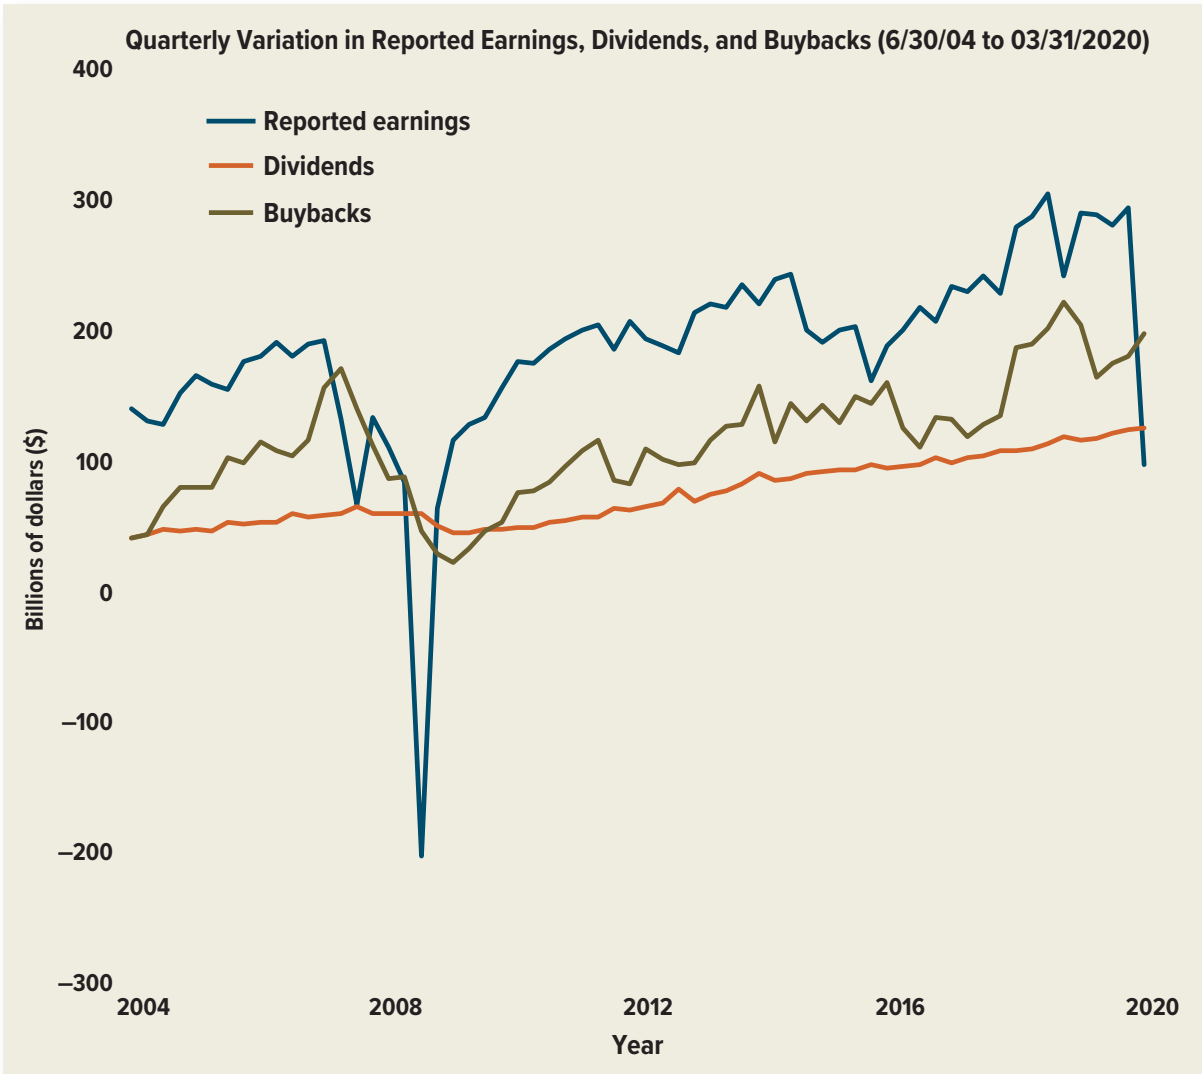
\includegraphics[width=0.6\textwidth]{images/section5/eds}
\end{figure}

\tiny{Source: Federal Reserve, via CFA Institute (through 03/31/2020)}

\end{frame}
\begin{frame}{Dividend vs. Stock Repurchase}{Original Balance Sheet}
	Consider a firm that wishes to distribute \$100,000 to its shareholders.
% Please add the following required packages to your document preamble:
% \usepackage{booktabs}
\begin{table}[]
	\begin{tabular}{@{}lrlr@{}}
		\multicolumn{2}{l}{\textit{\textbf{Assets}}} & \multicolumn{2}{l}{\textit{\textbf{Liabilities   \& Equity}}} \\
		\multicolumn{2}{l}{A. Original   balance sheet} &  & \multicolumn{1}{l}{} \\ \midrule
		Cash & \multicolumn{1}{r|}{\$150,000} & Debt & 0 \\
		Other Assets & \multicolumn{1}{r|}{\$850,000} & Equity & \$1,000,000 \\
		Value of Firm & \multicolumn{1}{r|}{\$1,000,000} & Value of Firm & \$1,000,000 \\ \bottomrule
	\end{tabular}
\end{table}
\begin{itemize}
	\item Shares outstanding = 100,000
	\item Price per share = \$1,000,000 / 100,000 = \$10
\end{itemize}
\end{frame}

\begin{frame}{Dividend vs. Stock Repurchase}{After Dividend Payment (Stock Price Falls)}
	If they distribute the \$100,000 as a cash dividend, the balance sheet will look like this:
	% Please add the following required packages to your document preamble:
	% \usepackage{booktabs}
	\begin{table}[]
		\begin{tabular}{@{}lrlr@{}}
			\multicolumn{2}{l}{\textit{\textbf{Assets}}} & \multicolumn{2}{l}{\textit{\textbf{Liabilities   \& Equity}}} \\
			\multicolumn{2}{l}{B. After \$1 per share cash dividend} &  & \multicolumn{1}{l}{} \\ \midrule
			Cash & \multicolumn{1}{r|}{\$50,000} & Debt & 0 \\
			Other Assets & \multicolumn{1}{r|}{\$850,000} & Equity & \$900,000 \\
			Value of firm & \multicolumn{1}{r|}{\$900,000} & Value of firm & \$900,000 \\ \bottomrule
		\end{tabular}
	\end{table}
\begin{itemize}
\item Shares outstanding = 100,000
\item Price per share = \$900,000 / 100,000 = \$9
\end{itemize}
\end{frame}

\begin{frame}{Dividend vs. Stock Repurchase}{After Stock Repurchase (Stock Price Stable, Shares Reduce)}
If they distribute the \$100,000 through a stock repurchase, the balance sheet will look like this:
% Please add the following required packages to your document preamble:
% \usepackage{booktabs}
\begin{table}[]
	\begin{tabular}{@{}lrlr@{}}
		\multicolumn{2}{l}{\textit{\textbf{Assets}}} & \multicolumn{2}{l}{\textit{\textbf{Liabilities   \& Equity}}} \\
		\multicolumn{2}{l}{C.  After stock repurchase} &  & \multicolumn{1}{l}{} \\ \midrule
		Cash & \multicolumn{1}{r|}{\$50,000} & Debt & 0 \\
		Other Assets & \multicolumn{1}{r|}{\$850,000} & Equity & \$900,000 \\
		Value of firm & \multicolumn{1}{r|}{\$900,000} & Value of firm & \$900,000 \\ \bottomrule
	\end{tabular}
\end{table}
\begin{itemize}
	\item Shares outstanding = 90,000
	\item Price per share = \$900,000 / 90,000 = \$10
\end{itemize}
\end{frame}
\begin{frame}{Dividend vs. Repurchase: Key Insight}

\begin{itemize}
    \item In a perfect market (no taxes, transaction costs, or signaling effects), \textbf{dividends and repurchases are equivalent}.
    \item Key difference:
    \begin{itemize}
        \item \textbf{Dividends} reduce cash and equity; share price falls.
        \item \textbf{Repurchases} reduce cash and shares; share price stays the same.
    \end{itemize}
    \item Choice between them depends on taxes, signaling, flexibility, and incentives.
\end{itemize}

\end{frame}

\begin{frame}{Why Do Firms Prefer Repurchases?}

\textbf{1. Flexibility}
\begin{itemize}
    \item Dividends are viewed as commitments; cuts are penalized.
    \item Repurchases offer temporary, non-binding payouts.
\end{itemize}

\vspace{2mm}
\textbf{2. Managerial Incentives}
\begin{itemize}
    \item Repurchases increase EPS and stock price -- both favorable to option-holding executives.
    \item Firms use repurchases to offset dilution from equity compensation.
\end{itemize}

\end{frame}

\begin{frame}{Why Do Firms Prefer Repurchases? (cont'd)}

\textbf{3. Signaling}
\begin{itemize}
    \item Repurchase announcements often interpreted as \textit{"we believe our stock is undervalued"}.
\end{itemize}

\vspace{2mm}
\textbf{4. Tax Efficiency}
\begin{itemize}
    \item Capital gains from repurchases are taxed more favorably than dividends in many jurisdictions.
\end{itemize}

\vspace{2mm}
\textbf{5. Takeover Defense}
\begin{itemize}
    \item Repurchases reduce shares available to potential hostile acquirers.
\end{itemize}

\end{frame}

\begin{frame}{Summary: Dividend vs. Share Repurchase}

\begin{table}[ht]
\centering
\resizebox{\linewidth}{!}{
\begin{tabular}{l >{\raggedright\arraybackslash}p{4.5cm} >{\raggedright\arraybackslash}p{6.5cm}}
\toprule
\textbf{Dimension} & \textbf{Dividends} & \textbf{Share Repurchases} \\
\midrule
\textbf{Flexibility} & Typically viewed as a long-term commitment & More flexible, can be adjusted based on cash flows \\
\textbf{Signal to Market} & May signal confidence if increased & Often viewed as a signal of undervaluation \\
\textbf{Tax Treatment} & Taxed as dividend income (often higher) & Taxed as capital gains (usually lower) \\
\textbf{Effect on Share Price} & Share price drops on ex-dividend date & Share price often unchanged, but EPS increases \\
\textbf{Impact on Share Count} & No change in shares outstanding & Reduces shares outstanding, increases ownership concentration \\
\textbf{Effect on Management Incentives} & Less direct impact on stock options & May increase value of outstanding stock options \\
\bottomrule
\end{tabular}
}
\end{table}

\end{frame}

\subsection{Personal Taxes and Payout Policy}
\begin{frame}{Personal Taxes and Payout Policy}
    \begin{itemize}
        \item The irrelevance of dividend policy relies on idealized assumptions:
        \begin{itemize}
            \item No taxes
            \item No transaction costs
            \item No uncertainty
        \end{itemize}
        \item In practice, taxes introduce important frictions:
        \begin{itemize}
            \item In \textbf{China}:
            \begin{itemize}
                \item Cash dividends are taxed at \textbf{20\%}.
                \item Capital gains tax exists but is not always enforced.
            \end{itemize}
            \item In the \textbf{U.S.}:
            \begin{itemize}
                \item Both dividends and capital gains are taxed at \textbf{15\%}.
                \item \textit{Capital gains are deferrable}—effective tax rate is lower.
            \end{itemize}
        \end{itemize}
        \item Bottom line: \textbf{Dividends are typically taxed more heavily than capital gains}.
    \end{itemize}
\end{frame}

\begin{frame}{Payouts with No Taxes}
    \begin{itemize}
        \item Suppose a firm distributes dividends but lacks sufficient cash.
        \item The firm raises funds via stock issuance and returns those funds as dividends.
        \item \textbf{Result:} A complete wash -- no change in shareholder wealth.
    \end{itemize}
    \begin{figure}
        \centering
        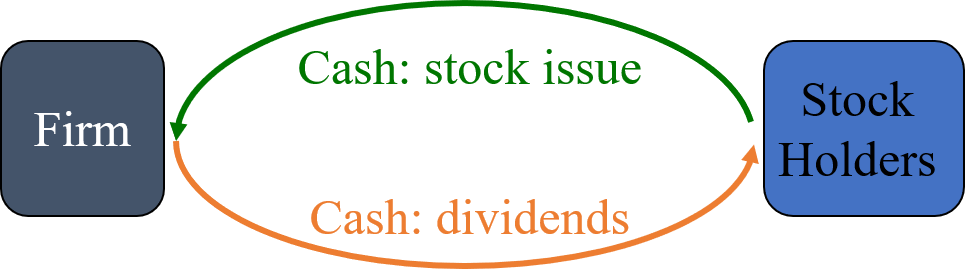
\includegraphics[width=0.65\textwidth]{images/section5/firmwithout1.png}
    \end{figure}
\end{frame}

\begin{frame}{Payouts with Taxes: Destroying Value}
    \begin{itemize}
        \item Now assume a \textbf{15\% tax} on dividends.
        \item Issuing shares to pay dividends incurs a tax burden on shareholders.
        \item \textbf{Conclusion:} This strategy reduces overall value and is dominated by doing nothing.
    \end{itemize}
    \begin{figure}
        \centering
        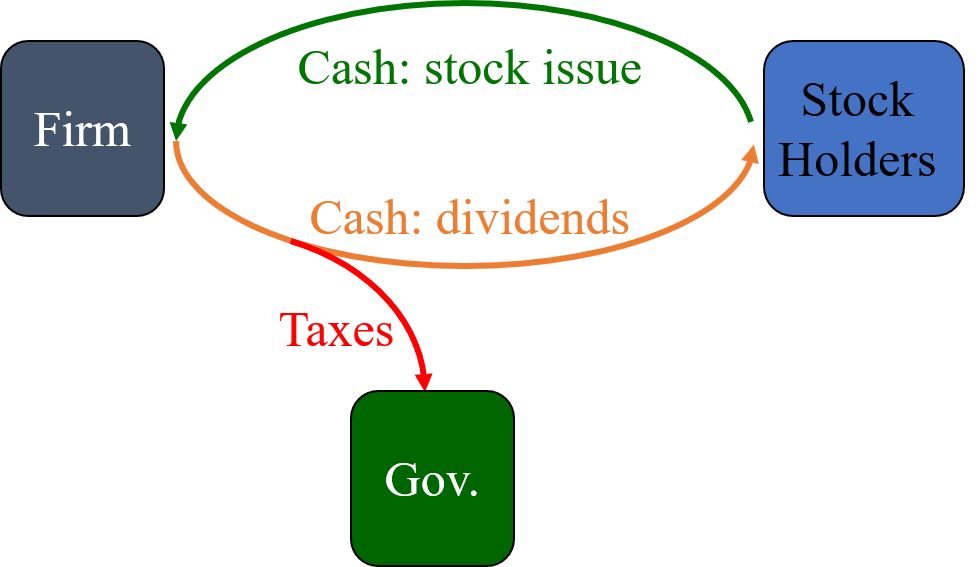
\includegraphics[width=0.65\textwidth]{images/section5/firmwithout2.png}
    \end{figure}
\end{frame}

\begin{frame}{Payouts with Taxes + Transaction Costs}
    \begin{itemize}
        \item In addition to tax inefficiency, \textbf{stock issuance incurs fees}.
        % \item Investment banks and legal expenses reduce the firm's remaining value.
        % \item \textbf{Lesson:} Never issue equity just to pay dividends.
    \end{itemize}
    \begin{figure}
        \centering
        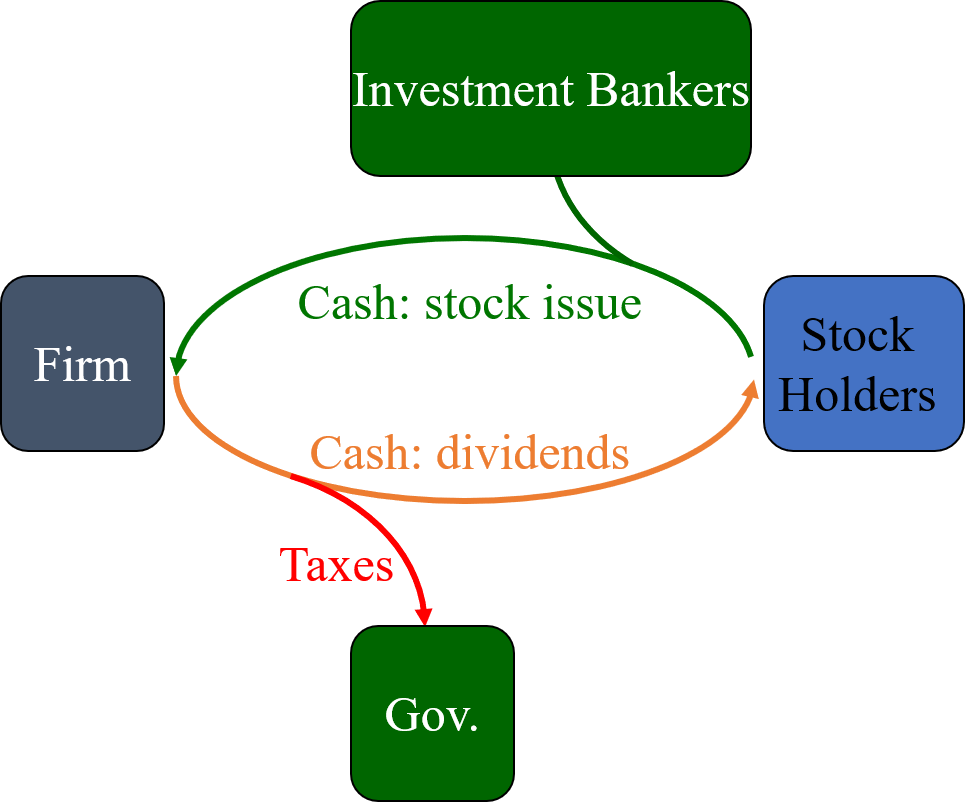
\includegraphics[width=0.65\textwidth]{images/section5/firmwithout3.png}
    \end{figure}
\end{frame}

\begin{frame}{When Firms Have Excess Cash}
    \begin{itemize}
        \item Tax arguments apply differently when the firm has extra cash \textbf{after investing in all positive NPV projects}.
        \item Options for excess funds:
        \begin{itemize}
            \item Take on negative NPV projects (value destroying)
            \item Acquire firms or buy financial assets
            \item Distribute cash via \textbf{dividends or share repurchases}
        \end{itemize}
        \item \textbf{Best practice:} return excess capital to shareholders unless a superior use exists.
    \end{itemize}
\end{frame}
\begin{frame}{Dividend Timing and Tax Efficiency}
    \begin{block}{Example: Regional Electric Company}
        Regional Electric has \$1,000 of excess cash. It can either:
        \begin{enumerate}
            \item Pay the amount as a \textbf{dividend now}, or
            \item \textbf{Retain and invest} it in 10\% Treasury bills, paying a dividend after 5 years.
        \end{enumerate}
        \vspace{0.2cm}
        \textbf{Assumptions:}
        \begin{itemize}
            \item Corporate tax rate: 21\%
            \item Personal tax rate on interest: 28\%
            \item Dividend tax rate: 15\%
            \item Investors can also invest in 10\% Treasury bills directly
        \end{itemize}
        \textbf{Question:} Which policy leaves investors better off after 5 years?
    \end{block}
\end{frame}
\begin{frame}{After-Tax Wealth: Immediate vs Deferred Dividend}
    \begin{itemize}
        \item \textbf{Option 1: Pay dividend now}
        \begin{itemize}
            \item Dividend received: \$1,000 × (1 - 15\%) = \$850
            \item Invest at 10\% for 5 years, taxed at 28\%:
            \[
            \$850 \times \left[1 + 0.10 \times (1 - 0.28)\right]^5 = \text{\$1,203.35}
            \]
        \end{itemize}

        \vspace{0.3cm}
        \item \textbf{Option 2: Retain cash, invest in T-bills, pay dividend in Year 5}
        \begin{itemize}
            \item Corporate investment grows at after-tax return:
            \[
            \$1,000 \times \left[1 + 0.10 \times (1 - 0.21)\right]^5 = \text{\$1,462.54}
            \]
            \item Dividend taxed at 15\% in Year 5:
            \[
            \$1,462.54 \times (1 - 0.15) = \text{\$1,243.16}
            \]
        \end{itemize}

        \vspace{0.3cm}
        \item \textbf{Conclusion:} Deferring the dividend results in greater after-tax wealth:  
        \textbf{\$1,243.16 vs. \$1,203.35}
    \end{itemize}
\end{frame}

\begin{frame}{Summary: Personal Taxes and Payout Policy}
	\begin{itemize}
		\item \textbf{In a world with personal taxes:}
		\begin{itemize}
			\item Firms should \textbf{not issue equity to pay dividends} -- this is inefficient due to double taxation.
			\item Managers have incentives to minimize dividend payments by seeking alternative uses for cash:
			\begin{itemize}
				\item Invest in capital expenditures (CAPEX)
				\item Pursue M\&A opportunities
				\item Accumulate financial assets (e.g., T-bills)
			\end{itemize}
			\item However, \textbf{practical limits} on these activities often leave firms with excess cash -- resulting in residual dividend payments.
		\end{itemize}
		\vspace{0.2cm}
		\item \textbf{Key tension:}  
		Personal taxes reduce the attractiveness of dividends, yet most firms continue to pay them.
		
		\item \textbf{Open puzzle:}  
		Why do firms \textit{prefer dividends} over tax-efficient share repurchases?
	\end{itemize}
\end{frame}

\subsection{Real-World Factors Favoring High Dividends}
\begin{frame}{Why Firms Might Favor High Dividends}
	\begin{itemize}
		\item \textbf{Investor Preference for Current Income} -- Especially retirees or income-focused investors.
		\item \textbf{Behavioral Factors} -- Dividends act as a self-control device for spending.
		\item \textbf{Agency Costs} -- Paying dividends reduces managerial discretion over free cash flow.
		\item \textbf{Information Content and Signaling} -- Dividend changes convey management's private information.
	\end{itemize}
\end{frame}

\subsubsection{Investor Preference, Behavioral Finance and Clientele Effect}
\begin{frame}{Investor Preference for Current Income}
\footnotesize
\begin{itemize}
    \item \textbf{Some investors -- particularly retirees -- prioritize stable cash flows} to fund consumption without selling shares.

    \item \textbf{In theory}: With no taxes or frictions, dividends and share sales are equivalent -- investors could create "homemade dividends."

    \item \textbf{In practice}:
    \begin{itemize}
        \item Selling shares involves \textit{transaction costs}, \textit{capital gains taxes}, and \textit{timing risk}.
        \item Dividends offer convenience, simplicity, and predictable cash flow.
    \end{itemize}

    \item \textbf{Conclusion:} Demand for dividends from income-oriented investors may push up the prices of high-dividend stocks.
\end{itemize}
\end{frame}

\begin{frame}{Behavioral Finance: Self-Control and Dividend Demand}
\footnotesize
\begin{itemize}
    \item \textbf{Self-control problems} can lead investors to overconsume or mismanage withdrawals from investments.

    \item Two strategies to generate income:
    \begin{itemize}
        \item \textbf{Dividend discipline:} Consume only what is paid as dividends -- automatic budgeting.
        \item \textbf{Self-liquidation:} Sell shares as needed -- requires restraint and active decision-making.
    \end{itemize}

    \item \textbf{Behavioral insight:} Regular dividends act as a commitment device, helping avoid temptation and poor timing.

    \item \textbf{Implication:} Even if inefficient in theory, dividends may enhance welfare by supporting investor discipline.
\end{itemize}
\end{frame}

\begin{frame}{From Self-Control to Clientele Effects}
\footnotesize
\begin{itemize}
    \item \textbf{Behavioral motivations, like self-control, help explain why some investors prefer dividends.}
    
    \item But dividend demand isn't driven by behavior alone.
    \begin{itemize}
        \item Taxes, income needs, and institutional constraints also play a role.
    \end{itemize}
    
    \vspace{0.2cm}
    \item \textbf{Together, these factors form the basis of the \textit{Dividend Clientele Hypothesis}}:
    \begin{itemize}
        \item Different investor groups prefer different payout policies.
        \item Firms may shape or respond to the makeup of their shareholder base accordingly.
    \end{itemize}
    
    \vspace{0.2cm}
    \item \textbf{Next:} We explore who prefers what -- and why -- in dividend clientele formation.
\end{itemize}
\end{frame}

\begin{frame}{The Dividend Clientele Effect}
\footnotesize
\begin{itemize}
    \item \textbf{Investor preferences vary by tax status and income needs} -- creating distinct "clienteles" for dividend policies.
\end{itemize}

\vspace{0.2cm}
\begin{table}[h]
	\centering
	\small
    \begin{tabular}{ll}
		\toprule
		\textbf{Investor Group} & \textbf{Preferred Payout Policy} \\
		\midrule
		High-Tax Individuals & Low or No Dividends \\
		Retirees / Income-Seekers & Moderate to High Dividends \\
		Tax-Exempt Institutions & Indifferent or High Dividends \\
		Corporations & High Dividends (due to inter-corporate exemption) \\
		\bottomrule
	\end{tabular}
	
\end{table}

\vspace{0.2cm}
\begin{itemize}
    \item \textbf{Implication:} Firms may tailor payout policy to attract or retain their target shareholder base.
\end{itemize}
\end{frame}

\begin{frame}{Retail Investor Preferences: Empirical Evidence}
\footnotesize
\begin{itemize}
    \item Surveys and trading data show that \textbf{many individual investors prefer high-dividend stocks}.
    \item This preference persists despite theoretical arguments for dividend irrelevance.
\end{itemize}

\begin{figure}
    \centering
    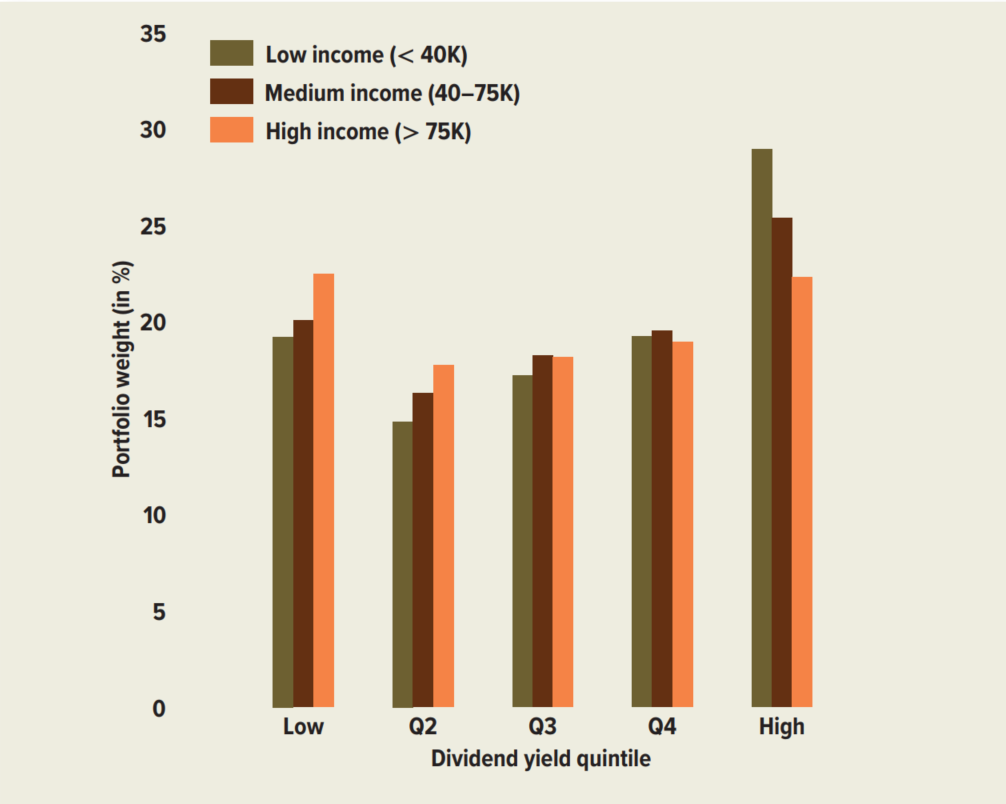
\includegraphics[height=0.5\textheight]{images/section5/dividendyield}
\end{figure}

\tiny{Source: \textcite{graham2006dividend}. Retail investors reveal a bias toward high dividend yields in portfolio choices.}
\end{frame}

\begin{frame}{Summary: Behavioral and Clientele Effects}
\begin{figure}
    \centering
    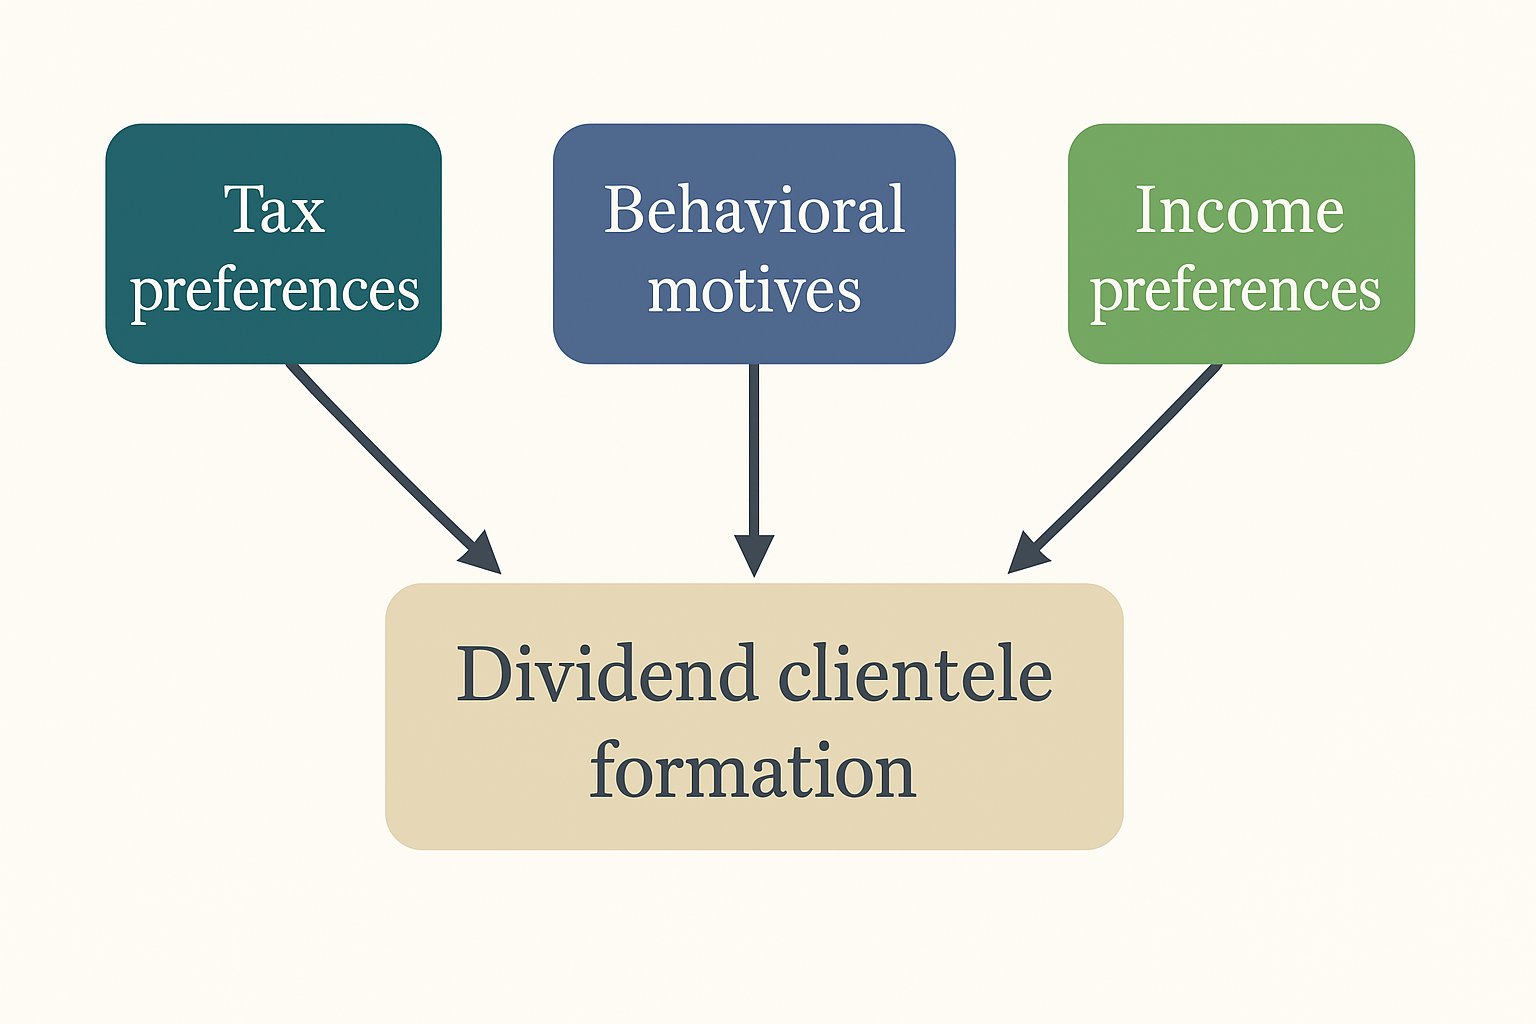
\includegraphics[width=0.8\linewidth]{images/section5/clientele.png}
\end{figure}
\end{frame}

\subsubsection{Dividends and Agency Costs}
\begin{frame}{Dividends and Agency Costs}
\footnotesize
\begin{itemize}
    \item \textbf{Agency Conflict:} Managers may pursue inefficient investments, perks, or empire-building when excess cash is available.
    
    \vspace{1mm}
    \item \textbf{Role of Dividends:}
    \begin{itemize}
        \item Reduces \textbf{free cash flow} under managerial discretion.
        \item Forces managers to return capital to shareholders rather than reinvest wastefully.
    \end{itemize}
    
    \vspace{1mm}
    \item \textbf{Additional Effects:}
    \begin{itemize}
        \item May \textit{transfer wealth from bondholders to shareholders} during financial distress.
        \item Acts as a \textbf{signal} that management prioritizes shareholder interests.
    \end{itemize}
    
    \vspace{1mm}
    \item \textbf{Implication:} Dividend policy can serve as a governance mechanism in firms with high free cash flow.
\end{itemize}
\end{frame}

\subsubsection{Information Content of Dividends and Dividend Signaling}

\begin{frame}{Information Content of Dividends}
\footnotesize
\begin{itemize}
    \item Dividend changes convey management's private information about future performance:
    \begin{itemize}
        \item \textbf{Increase} $\rightarrow$ signal of expected stronger future cash flows and earnings
        \item \textbf{Decrease} $\rightarrow$ often interpreted as a sign of financial weakness
    \end{itemize}

    \vspace{2mm}
    \item Academic evidence supports this view:
    \begin{itemize}
        \item \textcite{asquith1983impact} and \textcite{michaely1995price} show positive abnormal returns following dividend increases, and negative returns after cuts.
    \end{itemize}

    \item \textbf{Takeaway:} The stock market reacts not just to the amount of dividends, but to the information embedded in changes to dividend policy.
\end{itemize}
\end{frame}

\begin{frame}{Dividend Signaling: Why It's Credible}
\footnotesize
\begin{itemize}
    \item \textbf{Can firms "fake" strong performance by raising dividends?}
    \begin{itemize}
        \item In the short term, yes -- but only at a cost.
        \item Higher dividends must be paid in cash -- real money, not just promises.
    \end{itemize}

    \vspace{2mm}
    \item \textbf{Why is the signal credible?}
    \begin{itemize}
        \item Firms with weak earnings cannot sustain elevated payouts without jeopardizing liquidity or future investment.
        \item This cost makes it unattractive for low-quality firms to mimic high-quality ones.
    \end{itemize}

    \vspace{2mm}
    \item \textbf{Implication:} Only firms with strong future prospects raise dividends, making dividend increases a \textbf{credible signal}.
\end{itemize}
\end{frame}

\begin{frame}{Dividend Announcement and Market Inference (I)}
\footnotesize
\textbf{Assumption:}  
Firm is all-equity financed. Identity:
\[
\text{Cash Flow} = \text{CapEx} + \text{Dividends}
\]

\vspace{2mm}
\textbf{Scenario A:}
\begin{itemize}
    \item Firm announces CapEx = \$80 million
    \item Market believes Cash Flow = \$130 million
    \item $\Rightarrow$ Market infers Dividend = \$50 million
\end{itemize}

\vspace{2mm}
\textbf{Scenario B:}
\begin{itemize}
    \item Firm announces Dividend = \$70 million (higher than expected)
    \item Market assumes Cash Flow unchanged (\$130M) $\rightarrow$ CapEx = \$60M
    \item Market reacts negatively $\rightarrow$ assumes profitable investment opportunities are being sacrificed
\end{itemize}
\end{frame}

\begin{frame}{Dividend Announcement and Market Inference (II)}
\footnotesize
\textbf{Alternative Market Interpretation:}
\begin{itemize}
    \item CapEx = \$80M remains unchanged
    \item Dividend = \$70M implies Cash Flow = \$150M
    \item Market revises expectations upward $\rightarrow$ stock price rises
\end{itemize}

\vspace{2mm}
\textbf{Credibility Mechanism:}
\begin{itemize}
    \item If firm raises dividends but doesn't have the cash flow, it will have to cut CapEx or raise funds.
    \item The truth will eventually be revealed through realized cash flows.
    \item Hence, only firms with sustainable earnings can afford to send this signal.
\end{itemize}

\vspace{2mm}
\textbf{Conclusion:}  
Dividend increases are costly to fake $\rightarrow$ they function as a \textbf{credible and informative signal} of firm strength.
\end{frame}

\subsubsection*{Summary}
\begin{frame}{Summary: Real-World Drivers of High Dividend Policy}
\footnotesize
\begin{itemize}
    \item \textbf{Investor Preferences}
    \begin{itemize}
        \item Some investors (e.g., retirees) desire stable income $\rightarrow$ prefer dividend-paying stocks.
        \item Transaction costs, taxes, and behavioral self-control make dividends more appealing than homemade alternatives.
        \item \textit{Clientele effect:} Different groups prefer different payout policies -- firms may cater to them.
    \end{itemize}
    \item \textbf{Agency Considerations}
    \begin{itemize}
        \item Dividends reduce free cash flow, limiting managerial discretion and curbing inefficiencies.
        \item May shift value from bondholders to shareholders during distress.
    \end{itemize}
    \item \textbf{Information and Signaling}
    \begin{itemize}
        \item Dividend increases can signal future profitability.
        \item Signaling is \textbf{costly to fake} -- only high-quality firms can sustain higher payouts.
    \end{itemize}
    % \item \textbf{Takeaway:}  
    % Though dividends may appear irrelevant in theory, real-world frictions make them a powerful corporate policy tool.
\end{itemize}
\end{frame}

\subsection{How Firms Pay Dividends Today}
\begin{frame}{How Firms Pay Dividends Today: Global Trends and Stylized Facts}
\footnotesize
\begin{itemize}
    \item \textbf{Dividends remain central to corporate payouts} despite theories of irrelevance.
    \begin{itemize}
        \item Aggregate global payouts continue to rise -- surpassing \$1.7 trillion in 2024.
        \item But the share of dividend-paying firms has declined in developed markets like the U.S.
    \end{itemize}
    \item \textbf{Corporate payout behavior is shaped by three regularities:}
    \begin{itemize}
        \item Firms \textit{smooth dividends} over time and avoid cuts.
        \item Dividends reflect long-term commitment; repurchases offer short-term flexibility.
        \item Payout policy adapts to firm characteristics, market norms, and investor demand.
    \end{itemize}
    \item \textbf{Cross-country variation matters.}
    \begin{itemize}
        \item Tax policies, institutional ownership, and governance norms shape dividend behavior.
        \item \textit{China's evolving payout practices} offer a revealing contrast to Western models.
    \end{itemize}
\end{itemize}
\end{frame}


\begin{frame}{Dividends Remain Substantial in Practice}
\footnotesize
\begin{itemize}
    \item \textbf{Despite theoretical arguments for dividend irrelevance, aggregate dividend payouts have grown steadily over time.}
    
    \vspace{2mm}
    \item \textbf{Key evidence:}
    \begin{itemize}
        \item In the U.S., total dividends paid by listed firms more than tripled from the 1980s to the 2020s.
        \item Globally, dividends constitute a significant share of total equity returns.
    \end{itemize}
    
    \vspace{2mm}
    \item \textbf{Reasons dividends remain relevant:}
    \begin{itemize}
        \item Institutional investor demand (e.g., pension funds)
        \item Cultural and market expectations
        \item Managerial incentives tied to dividend performance
    \end{itemize}
\end{itemize}
\end{frame}

\begin{frame}{Global Dividend Payouts Reach Record \$1.75 Trillion in 2024}
% \footnotesize
% \begin{itemize}
%     \item Despite the rise of share repurchases and shifting investor preferences, global dividend payouts remain at record highs.
    
%     \item \textbf{In 2024, global dividends reached \$1.75 trillion}, driven by robust corporate profits and continued shareholder demand for income.
    
%     \item The chart (right) shows the steady upward trend in total global dividends over the past 15 years -- with notable resilience even during periods of global uncertainty (e.g., COVID-19).
    
%     \item \textbf{Key features:}
%     \begin{itemize}
%         \item Both regular and special dividends have grown substantially.
%         \item The post-pandemic recovery saw a particularly strong rebound in payouts.
%     \end{itemize}

%     \item \textbf{Source:} Janus Henderson Global Dividend Index (2025)
% \end{itemize}

\begin{figure}
    \centering
    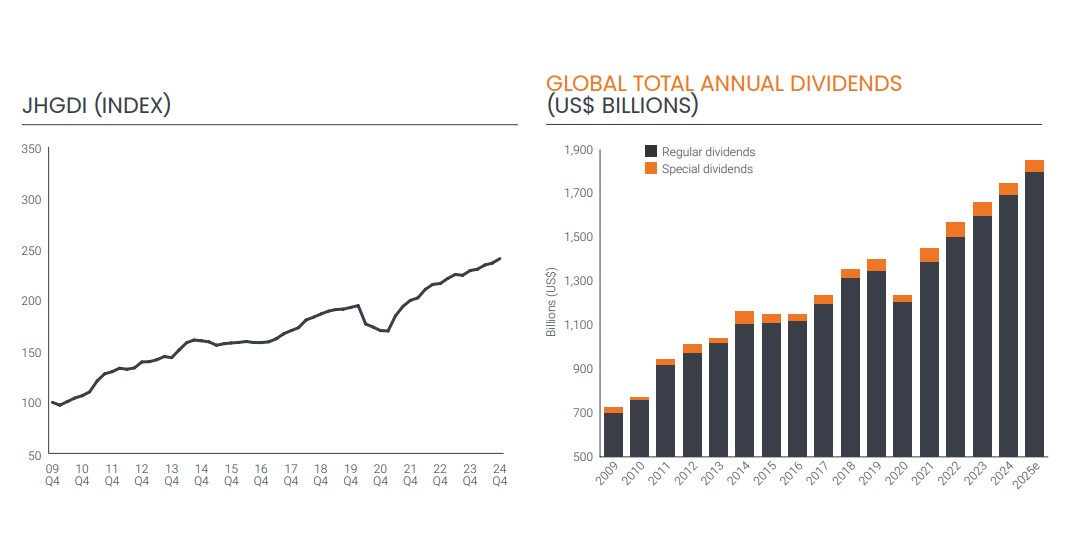
\includegraphics[width=0.85\linewidth]{images/section5/JHGDI.jpg}
\end{figure}
{\tiny
\textbf{Source:} Janus Henderson Global Dividend Index (2025) \url{https://www.fundssociety.com/en/news/markets/global-dividend-payouts-reach-record-1-75-trillion-in-2024/}}
\end{frame}

\begin{frame}{Dividends vs. Buybacks: S\&P 500 (1998-2020)}
\begin{figure}
    \centering
    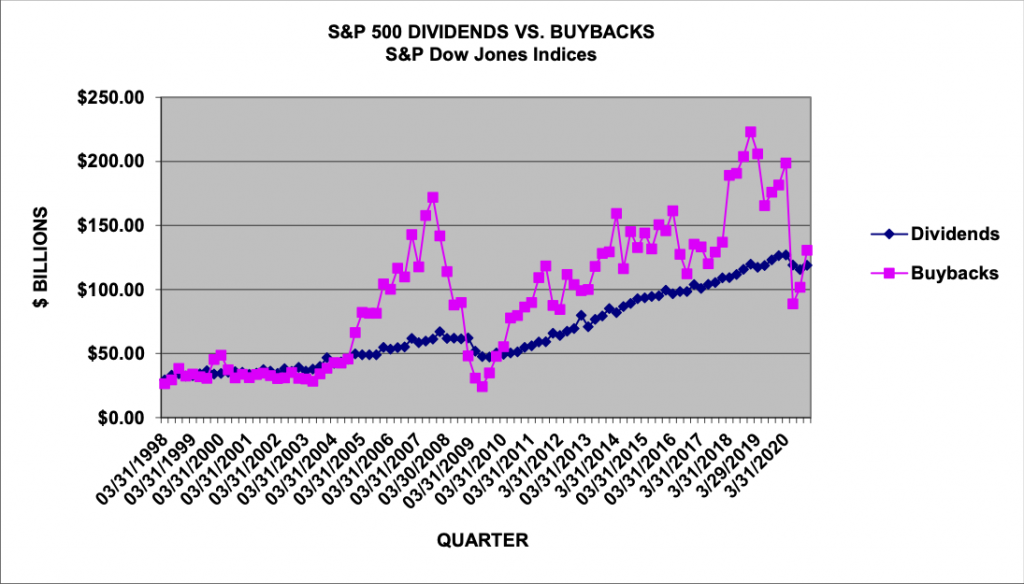
\includegraphics[width=0.95\linewidth]{images/section5/dividends_vs_buybacks.png}
\end{figure}
\tiny{Source: S\&P Dow Jones Indices. \url{https://dqydj.com/sp-500-dividend-yield/}}
\end{frame}

\begin{frame}{Trends in Corporate Payouts: Key Observations}
\footnotesize
\begin{itemize}
    \item \textbf{Both dividends and stock buybacks increased significantly} over the past two decades, but their patterns differ:
    \begin{itemize}
        \item Dividends grow steadily and predictably.
        \item Buybacks are more volatile -- firms ramp up repurchases during booms and cut them during downturns.
    \end{itemize}
    
    \vspace{2mm}
    \item \textbf{Since the mid-2000s, buybacks have often exceeded dividends}, indicating a shift in corporate payout preference.
    
    \vspace{2mm}
    \item \textbf{During economic shocks} (e.g., 2008 crisis, COVID-19 pandemic), companies generally preserve dividends but slash buybacks -- suggesting dividends are perceived as stronger signals of financial stability.
    
    \vspace{2mm}
    \item \textbf{Takeaway:} Dividends are viewed as long-term commitments; buybacks offer flexibility and are used more opportunistically.
\end{itemize}
\end{frame}

\begin{frame}{Dividend Smoothing: Lintner's Model}
\footnotesize
\begin{itemize}
    \item \textbf{\textcite{lintner1956distribution}} interviewed managers and found two consistent behaviors:
    \begin{itemize}
        \item Firms aim for a \textbf{target payout ratio} of earnings over the long run.
        \item Managers adjust dividends \textbf{gradually}, as they wait to confirm earnings changes are permanent.
    \end{itemize}

    \vspace{2mm}
    \item Dividend changes follow the adjustment model:
    \[
    D_1 - D_0 = s \times (t \cdot \text{EPS}_1 - D_0)
    \]
    where:
    \begin{itemize}
        \item $D_1$: dividend next year; $D_0$: dividend this year
        \item $t$: target payout ratio
        \item $s$: speed of adjustment ($0 < s \leq 1$)
    \end{itemize}

    \vspace{2mm}
    \item \textbf{Implication:} Dividend policy is \textit{sticky}, forward-looking, and resistant to transitory earnings fluctuations.
\end{itemize}
\end{frame}

\begin{frame}{Example: Applying Lintner's Smoothing Model}
\footnotesize
\begin{itemize}
    \item Calculator Graphics, Inc. (CGI) follows:
    \begin{itemize}
        \item Target payout ratio $t = 0.30$
        \item Speed of adjustment $s = 0.5$
    \end{itemize}

    \item \textbf{Year 1:}
    \begin{itemize}
        \item Last year's EPS = \$10, dividends = \$3.00
        \item This year's EPS = \$20
        \item Implied dividend change:
        \[
        \Delta D = 0.5 \times (0.30 \times 20 - 3.00) = 1.50
        \]
        \item New dividend = \$4.50
    \end{itemize}

    \item \textbf{Year 2:} EPS remains at \$20
    \begin{itemize}
        \item New target = \$6.00; current = \$4.50
        \item \[
        \Delta D = 0.5 \times (6.00 - 4.50) = 0.75
        \]
        \item New dividend = \$5.25
    \end{itemize}

    \item \textbf{Conclusion:} Dividend growth is \textit{deliberate and partial}, not a mechanical response to earnings.
\end{itemize}
\end{frame}

\begin{frame}{Chinese Firms: Rising Payouts and Policy Push}
\footnotesize
\begin{itemize}
    \item Chinese listed firms are increasing shareholder payouts under \textbf{regulatory pressure} and growing \textbf{investor demand for returns}.
    \item Reuters/LSEG data reported cash dividends by large and mid-cap Chinese companies reaching a record ¥3.4 trillion in 2023, with projected growth of 1.2\% in 2024 and 8.6\% in 2025.
    \begin{itemize}
        \item These figures cover a broad universe of Chinese-listed firms; A-share-only data may show different patterns.
    \end{itemize}
    \item \textbf{Key drivers:}
    \begin{itemize}
        \item \textit{Regulatory reform:} CSRC and SASAC have issued guidance encouraging stronger shareholder returns.
        \item \textit{Governance pressure:} Reducing idle cash improves capital discipline.
        \item \textit{Investor demand:} Income-seeking investors and dividend ETF flows reinforce the trend.
    \end{itemize}
    \item \textbf{Bottom line:} China's payout policy is increasingly shaped by policy reform, governance concerns, and investor-return pressure.
\end{itemize}
\end{frame}

\begin{frame}{Dividend Payout Trends in China}
\centering
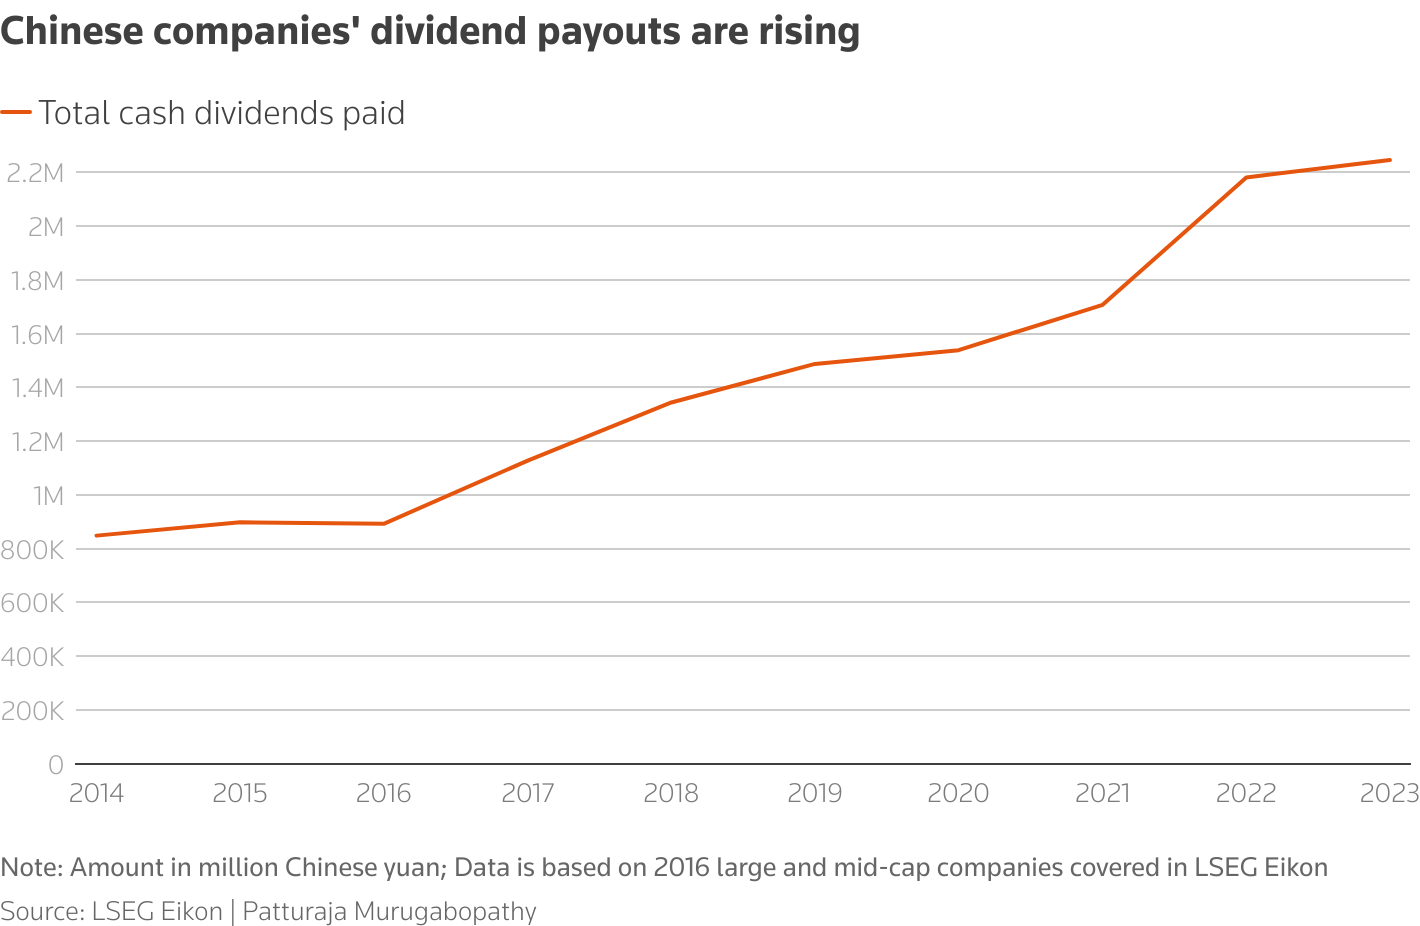
\includegraphics[width=0.75\linewidth]{images/section5/cndprising.png}

\vspace{1mm}
\begin{flushleft}
\scriptsize
\textit{Note:} Data are based on aggregate Chinese-listed companies through approximately 2023. The trend reflects improving cash-return practices; it does not imply all firms are mature dividend payers.
\end{flushleft}
\end{frame}

\begin{frame}{Dividend Payout Ratio: China vs. Other Asian Markets}
\centering
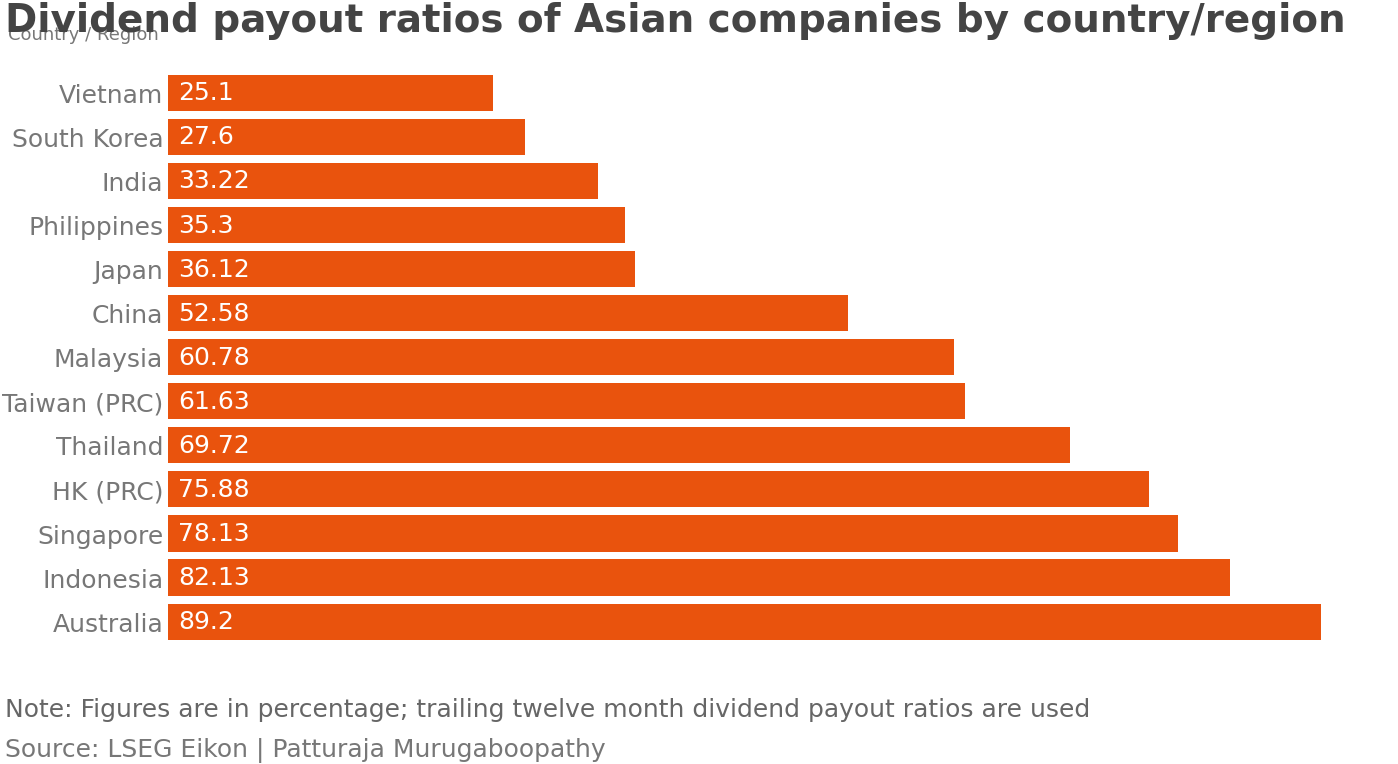
\includegraphics[width=0.65\linewidth]{images/section5/dprbycountry.png}

\vspace{1mm}
\footnotesize
\begin{itemize}
    \item China's payout ratio (52.6\% at end-2023) exceeds Korea, Japan, and India, but trails Singapore, Hong Kong, and Indonesia.
    \item \textbf{Caveat:} Cross-country comparisons reflect differences in industry mix, state ownership, the weight of financial firms, and profitability cycles -- not just payout choices.
    \item Key takeaway: \textbf{China is no longer simply a low-payout market}.
\end{itemize}
\end{frame}

\begin{frame}[t]{China A-Shares: Buybacks Are Rising}
\centering
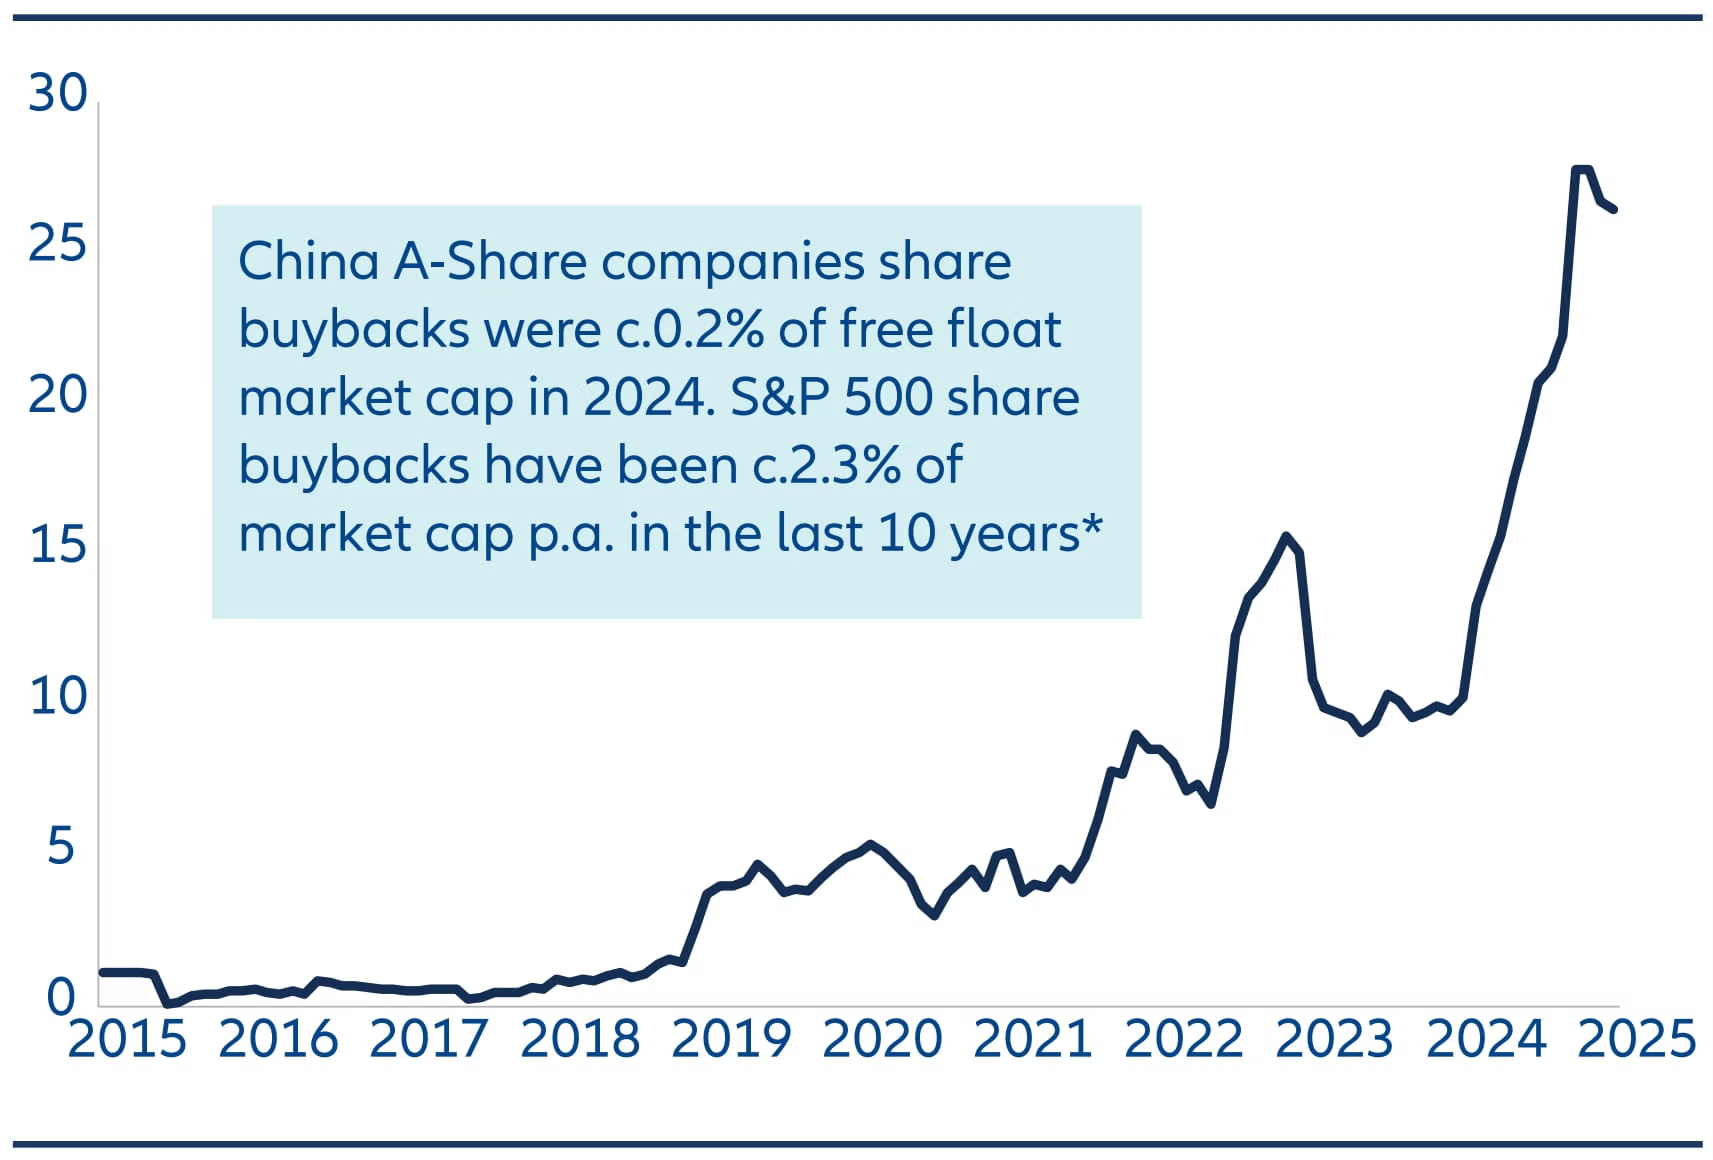
\includegraphics[width=0.68\textwidth]{images/section5/cn_buyback.png}

\vspace{-1mm}
\begin{flushleft}
\footnotesize
\begin{itemize}
    \item Buybacks have become a more visible payout channel in China.
    \item Regulatory encouragement and compressed valuations contributed to the surge in 2024.
\end{itemize}
{\scriptsize Source: Wind / Allianz Global Investors, as of Jan.\ 31, 2025; AllianzGI (2025).}
\end{flushleft}
\end{frame}

\begin{frame}[t]{China Equities: Cash Holdings and Payout Capacity}
\footnotesize
\begin{figure}
    \centering
    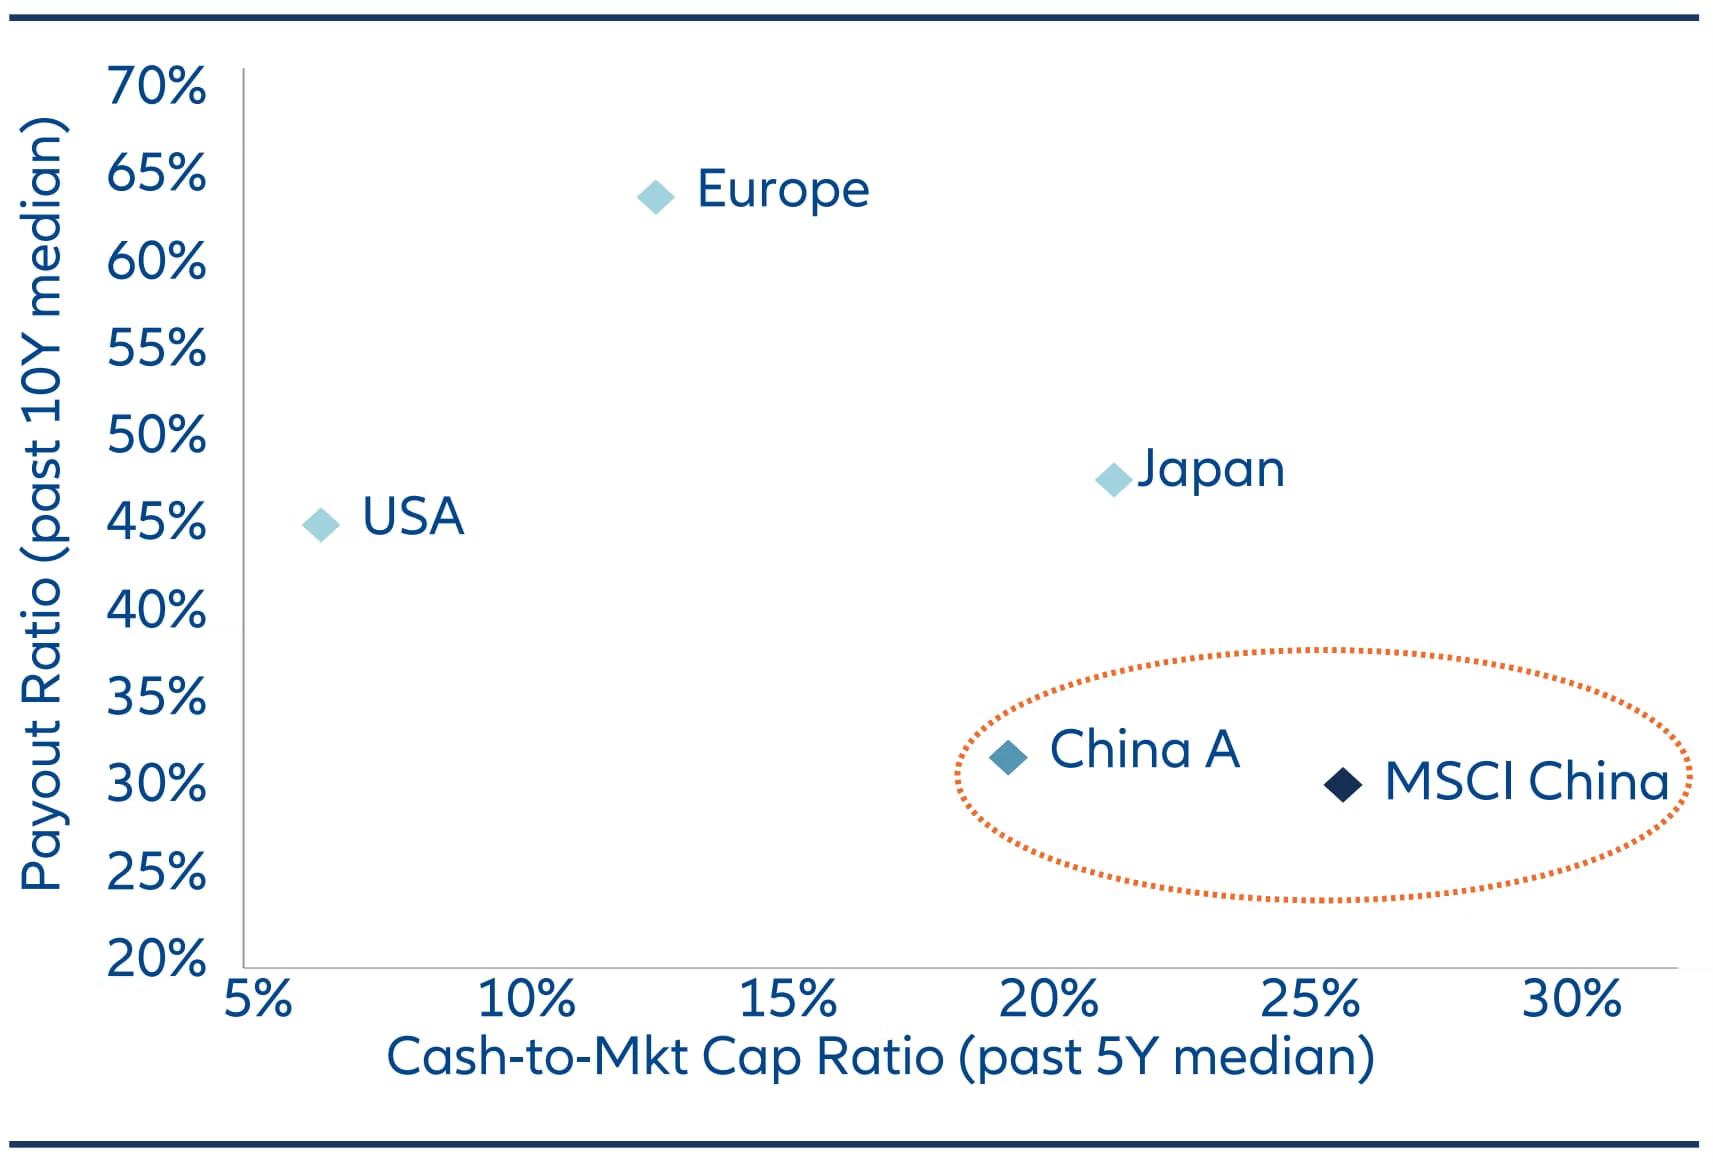
\includegraphics[width=0.62\textwidth]{images/section5/cn_dividend.png}
\end{figure}

\vspace{-0.25cm}

\begin{alertblock}{Interpretation}
Chinese firms hold substantial cash relative to market value, suggesting
room for higher dividends or repurchases. But payout capacity is not the
same as optimal payout.
\end{alertblock}

\vspace{-0.1cm}

{\scriptsize Source: Goldman Sachs, as of Apr.\ 25, 2024; reproduced in AllianzGI (2025).}

\end{frame}

\begin{frame}[t]{Investor Demand: Dividend ETF Inflows}
\footnotesize
\vspace{-0.1cm}
\begin{figure}
    \centering
    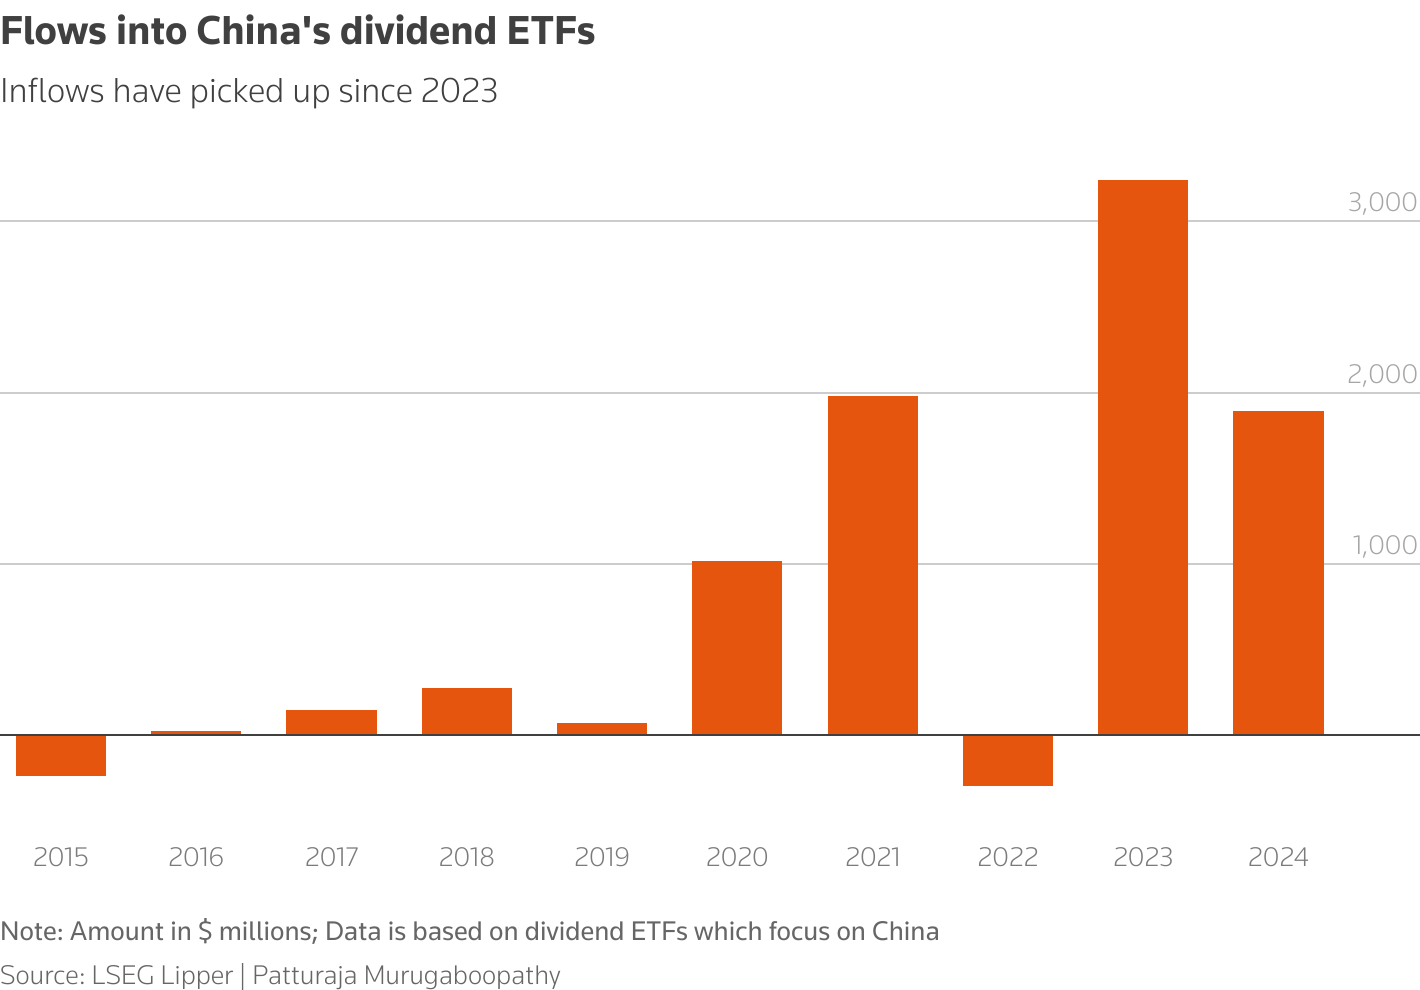
\includegraphics[width=0.64\linewidth]{images/section5/flowintocnde.png}
\end{figure}

\vspace{-0.25cm}

\begin{alertblock}{Interpretation}
Inflows into China dividend ETFs have accelerated since 2020, reflecting
stronger investor demand for cash returns and defensive equity exposure.
\end{alertblock}

{\scriptsize Source: Reuters / LSEG Lipper, based on dividend ETFs mainly focused on China.}

\end{frame}

\begin{frame}{Low Valuations Enhance Dividend Appeal}
\footnotesize
\begin{itemize}
    \item Chinese equities trade at \textasciitilde{}13x forward earnings -- below the S\&P 500 (\textasciitilde{}25x) and Nikkei 225 (\textasciitilde{}15x).
    \item Over 40 Chinese firms have dividend yields higher than their P/E ratios.
    \item Low valuations make dividend and buyback yields more salient; defensive, income-focused strategies gain appeal.
\end{itemize}
\centering
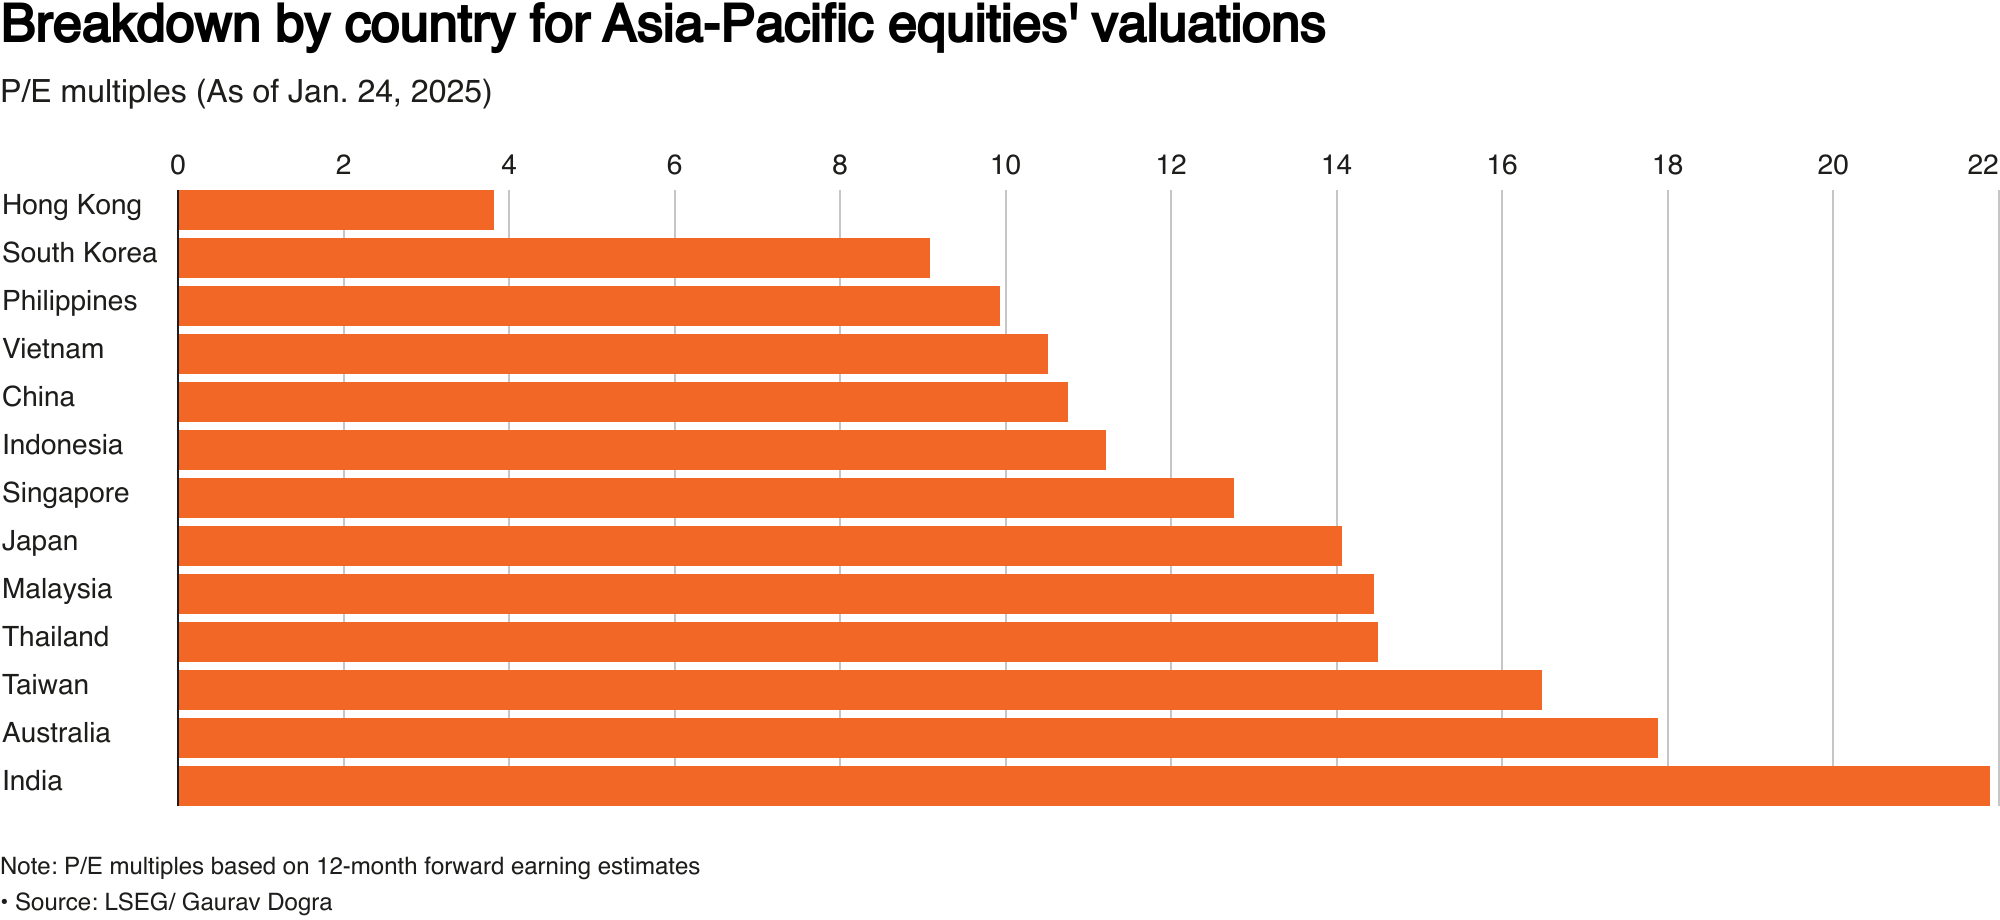
\includegraphics[width=0.85\linewidth]{images/section5/appe.png}
\end{frame}

\begin{frame}{China as a Payout Policy Case}
\footnotesize
\begin{itemize}
    \item \textbf{Governance channel:} Higher payouts reduce idle cash and improve shareholder discipline -- particularly relevant given state ownership and concentrated control.

    \item \textbf{Investor-demand channel:} Dividend ETFs and high-yield strategies attract investors seeking stable cash flows and defensive equity exposure.

    \item \textbf{Valuation channel:} Low valuations make dividend and buyback yields more salient; low prices reinforce the case for returning cash rather than retaining it.

    \item \textbf{Policy channel:} Regulators actively encourage stronger shareholder returns, shaping the institutional environment for rising payouts.
\end{itemize}
\vspace{2mm}
\begin{block}{}
\centering
\textit{China illustrates that payout policy is not only a firm-level decision; it is also shaped by market valuation, investor clientele, and regulatory reform.}
\end{block}
\end{frame}

\subsection{Payout Policy: Synthesis and Managerial Implications}
\begin{frame}{Why Dividends May Matter in Practice}
\footnotesize
\begin{itemize}
    \item \textbf{Investor Demand:} Appeals to income-seeking investors (e.g., retirees) who prefer stable cash flows without selling shares.
    
    \item \textbf{Behavioral Rationale:} Supports self-control -- investors avoid overspending by consuming only dividend income.
    
    \item \textbf{Agency Benefits:}
    \begin{itemize}
        \item Dividends reduce free cash flow available for managerial misuse ("overinvestment" problem).
        \item Limits resources that managers could divert toward empire building or perks.
    \end{itemize}

    \item \textbf{Signaling Value:} Dividend increases can signal management's confidence in future earnings.
\end{itemize}
\end{frame}

\begin{frame}{Costs and Limits of Cash Dividends}
\footnotesize
\begin{itemize}
    \item \textbf{Tax Inefficiency:} Dividends are taxed immediately, while capital gains are taxed only upon realization.

    \item \textbf{Reduced Financial Flexibility:}
    \begin{itemize}
        \item Dividends deplete internal capital.
        \item May force firms to forgo profitable projects or raise costly external equity.
    \end{itemize}

    \item \textbf{Sticky Commitment:} Once initiated, cutting dividends is difficult and often punished by the market.
    
    \item \textbf{Inflexible Tool:} Less adaptable to temporary changes in earnings compared to repurchases.

    \item \textbf{Shareholder--Creditor Conflict:} Large payouts in or near financial distress can transfer value from bondholders to shareholders. This is a value redistribution, not a firm-level benefit of dividends.
\end{itemize}
\end{frame}

\begin{frame}{Dividend Policy: Stylized Facts}
\begin{itemize}
    \item Aggregate corporate payouts (dividends + buybacks) have grown significantly over time.
    \item Dividends are paid primarily by large, mature, and profitable firms.
    \item Managers are reluctant to cut dividends -- they prefer to smooth payments.
    \item Stock prices respond to unexpected dividend changes (positive or negative).
    \item Repurchases are more volatile -- often tied to temporary earnings or stock price fluctuations.
\end{itemize}
\end{frame}

\begin{frame}{Managerial Guidelines for Payout Policy}

\begin{itemize}
    \item \textbf{Investment first:}
    Do not sacrifice positive-NPV projects to maintain or increase payouts.

    \item \textbf{Base regular dividends on sustainable cash flows:}
    Initiate dividends only when free cash flow is stable and predictable.

    \item \textbf{Smooth dividends:}
    Adjust regular dividends gradually, consistent with long-run earnings capacity.

    \item \textbf{Use repurchases for flexibility:}
    Buybacks are better suited for temporary excess cash or perceived undervaluation.

    \item \textbf{Consider taxes, clientele, and governance:}
    The optimal payout policy depends on investor preferences, tax treatment,
    agency problems, and financing constraints.
\end{itemize}

\vfill

\begin{alertblock}{Takeaway}
Payout policy should distribute excess cash without weakening investment
capacity, financial flexibility, or long-term firm value.
\end{alertblock}

\end{frame}

\subsection{Non-Cash Payouts: Stock Dividends and Stock Splits}

\begin{frame}{Non-Cash Payouts and Share Count Adjustments}
\begin{itemize}
    \item \textbf{Cash dividends:} Transfer cash from the firm to shareholders; firm value falls by the amount distributed.

    \item \textbf{Stock dividends:} Distribute additional shares to existing shareholders. No cash leaves the firm.

    \item \textbf{Stock splits:} Increase the number of shares and mechanically reduce price per share (e.g., a 2-for-1 split doubles share count and halves price).

    \item \textbf{Reverse splits:} Reduce the number of shares and mechanically increase price per share (e.g., a 1-for-10 reverse split).
\end{itemize}

\vspace{3mm}
\begin{block}{Key Idea}
Stock dividends, splits, and reverse splits change share count and per-share figures, but do \textbf{not} directly change total firm value.
\end{block}
\end{frame}

\begin{frame}{Peterson Co.: Stock Dividend Example}
\small
\textbf{Setup:} Peterson Co.\ declares a \textbf{10\% stock dividend}. Initial position: 10,000 shares at \$66/share (market cap \$660,000).

\vspace{3mm}
\begin{center}
\begin{tabular}{lccc}
\toprule
 & \textbf{Before} & \textbf{After} & \textbf{Change} \\
\midrule
Shares outstanding & 10,000 & 11,000 & $+$1,000 \\
Price per share & \$66.00 & \$60.00 & $-\$6.00$ \\
Market capitalization & \$660,000 & \$660,000 & None \\
\bottomrule
\end{tabular}
\end{center}

\vspace{2mm}
{\footnotesize Theoretical ex-price: $\$66 \times \frac{10{,}000}{11{,}000} \approx \$60.00$}

\vspace{2mm}
\begin{itemize}
    \item Total market value is mechanically unchanged.
    \item Each shareholder holds more shares, but each share is worth proportionally less.
    \item Proportional ownership is unchanged; no cash is distributed.
    \item \textit{Accounting note:} retained earnings are reclassified into paid-in capital --- no net equity change.
\end{itemize}
\end{frame}

\begin{frame}{Why Do Firms Split Shares?}
\begin{itemize}
    \item \textbf{Trading range:} Stocks priced too high may deter small investors. Splits keep the price in a psychologically or institutionally favorable range.

    \item \textbf{Perceived affordability:} A lower nominal price can attract retail investors and improve marketability.

    \item \textbf{Liquidity:} More shares at a lower price may improve bid-ask spreads and trading activity.

    \item \textbf{Reverse splits:} Used to avoid exchange delisting (e.g., Nasdaq's \$1 minimum price rule) or to eliminate administratively small shareholdings.
\end{itemize}

\vspace{3mm}
\begin{alertblock}{Caveat}
Splits are mostly cosmetic in valuation terms. Any lasting valuation effect must come from liquidity, signaling, or investor perception --- not from mechanical share-count changes.
\end{alertblock}
\end{frame}

\begin{frame}[t]{Stock Split vs.\ Large Stock Dividend}
\small
\begin{center}
\begin{tabular}{@{} l >{\raggedright\arraybackslash}p{3.6cm} >{\raggedright\arraybackslash}p{3.6cm} @{}}
\toprule
 & \textbf{Stock Split} & \textbf{Large Stock Dividend ($\geq 20\%$)} \\
\midrule
Share count      & Increases (e.g., $2\times$)  & Increases (e.g., $2\times$)  \\[2pt]
Price per share  & Falls proportionally          & Falls proportionally          \\[2pt]
Cash flow        & None                          & None                          \\[2pt]
Accounting       & Par value per share reduced; retained earnings unchanged & Retained earnings reclassified to paid-in capital (at par value) \\[2pt]
Total firm value & Unchanged                     & Unchanged                     \\
\bottomrule
\end{tabular}
\end{center}

\vspace{3mm}
\footnotesize \textbf{Example:} A 100\% stock dividend (one new share issued per share held) and a 2-for-1 split are economically equivalent --- the difference lies only in accounting treatment.
\end{frame}

\begin{frame}{Stock Dividends and Splits: Main Takeaway}
\begin{block}{}
\centering
Stock dividends and stock splits change the number of shares outstanding, but do \textbf{not} directly change total firm value.
\end{block}

\vspace{3mm}
\begin{itemize}
    \item \textbf{Cash dividends:} Distribute cash to shareholders; firm value falls.
    \item \textbf{Stock dividends:} Distribute shares; no cash leaves the firm.
    \item \textbf{Stock splits:} Mechanically lower price per share by increasing share count.
    \item \textbf{Reverse splits:} Mechanically raise price per share by reducing share count.
\end{itemize}

\vspace{3mm}
\begin{alertblock}{Practical Relevance}
These actions are mostly cosmetic in valuation terms, but they may matter for \textbf{liquidity}, \textbf{investor perception}, and \textbf{exchange listing requirements}.
\end{alertblock}
\end{frame}

\subsection*{Summary}
\begin{frame}{Summary: Dividends and Other Payouts}
\footnotesize
\begin{itemize}
  \item \textbf{Dividend Irrelevance (Theory)}: In perfect markets, payout policy does not affect firm value. Investors can create "homemade dividends."
  \item \textbf{Practical Frictions}:
  \begin{itemize}
    \item Taxes: Dividends are often taxed more heavily than capital gains.
    \item Agency issues: Dividends reduce managerial discretion over cash.
    \item Signaling: Dividend changes convey management's private information.
  \end{itemize}
  \item \textbf{Real-World Payout Practices}:
  \begin{itemize}
    \item Firms prefer to smooth dividends and avoid cuts.
    \item Share repurchases are more flexible and tax-efficient, increasingly favored.
    \item Payout decisions reflect investor preferences, corporate governance, and market norms.
  \end{itemize}
  \item \textbf{Stock Dividends and Splits}:
  \begin{itemize}
    \item Stock dividends and splits do not change total firm value.
    \item Often used to keep stock price in a desirable trading range or meet listing requirements.
  \end{itemize}
\end{itemize}
\end{frame}
